\documentclass[12pt,a4paper]{article}
\usepackage[latin1]{inputenc}
\usepackage{amsmath}
\usepackage{amsfonts}
\usepackage{amssymb}
\usepackage{graphicx}
\usepackage{float}
\usepackage{amsmath}
\usepackage{url}
\usepackage{hyperref}
\usepackage{listings}	% syntax highlight
\usepackage{verbatim}
\usepackage{minted}
\usepackage{pgfplots}
\usepackage{fix-cm}

\graphicspath{ {img/} }

\begin{document}

\begin{titlepage}
	\centering
	\vfill
	
\includegraphics[width=8cm]{upv_logo.png}
	
\includegraphics[width=8cm]{etsinf_logo.png}
	\vskip2cm
	
	{\fontsize{36}{30}\selectfont
		Open World Streaming:	
	}
	\linebreak
	{\huge
		
		Automatic memory management in open world games without loading screens.
	}
	\vskip2cm
	{\Large
		Alejandro Juan P�rez \\ \href{mailto:tuketet@gmail.com}{tuketet@gmail.com}\\
		\vskip1cm
		Supervised by\\Ram�n Pascual Moll� Vay�
		\vskip1cm
		2015-2016
	}   
\end{titlepage}

\newpage

\tableofcontents

\newpage

\section{Introduction}


Open world games are among the most appreciated games by players. They provide users the chance to explore a big world and they are very immersive.  Open world games grant players the freedom to take any decision and enjoy their high interaction.

In open world videogames the player, usually, controls an avatar over a big virtual world. So the player that controls the avatar takes its skin and, ideally, gets immersed in the virtual world.

There is a good chance you know about some of the most famous open world games. Some of them are: \emph{Grad Theft Auto} series \footnote{\emph{Grand Theft Auto} is a series of games produced by \emph{Rockstar}}
, \emph{The Elder Scrolls} series \footnote{\emph{The Elder Scrolls} is a series of games produced by \emph{Bethesda}} or
\emph{Minecraft} \footnote{\emph{Minecraft} is a sandbox game produced by \emph{Mojang}}.
These games, apart from being very famous, they have all been in the top of the best-selling videogames\cite{bestselling}.

\begin{itemize}
\item \emph{Minecraft} has sold 19 million copies for the PC platform and it is the most sold PC game ever.

\item \emph{Grand Theft Auto V} has sold 19 millons copies for the \emph{PS3}, making it the most sold \emph{PS3} game ever.

\item \emph{The Eder Scrolls: Skyrim} has sold 20 millon copies for \emph{PC}, \emph{XBOX} and \emph{PS3}.
\end{itemize}
  
Therefore, open world games are not only about fun, freedom and high interaction but also a promising business. And as we will see they are technologically challenging.

Despite open world games are well know, the techniques that are applied in their implementation are not. Game studios that are experienced in the implementation of open world games, like \emph{Rockstar}, keep well their secrets. The development of open world game engines requires a great investment.

The purpose of this project is to develop a game engine that will support making open world videogames. Our engine should allow the creation of games with huge worlds and avoid loading screens. There is very few information about the topic (specially at the implementation level). My intention is to gather available information and extend it with my own thoughts and get them to be implemented. Hopefully, this article, and the open source code that comes along with it, will help other people to understand the main concerns they should take when developing open world games.

\section{Open world videogames}

Open world are some kind of videogames in which the player can move freely in a huge virtual world. The structure of the game is not linear in terms of gameplay. That means, the player has the choice on what to do next. There are some game genres that can benefit a lot from the open world approach. For example, role playing games (RPG)\footnote{\url{https://en.wikipedia.org/wiki/Role-playing\_video\_game}}, sandbox\footnote{\url{https://en.wikipedia.org/wiki/Glossary\_of\_video\_game\_terms\#Sandbox\_game}} and vehicle simulation\footnote{\url{https://en.wikipedia.org/wiki/Vehicle\_simulation\_game}} are enhanced when convined with a big open world.

In some open world RPGs, the player can explore the world and complete missions. Some of these missions are not mandatory so the player is allowed to decide whether or not to take them. These is an example of the non-linearity we have been talking about.

\begin{figure}[H]
	\centering
	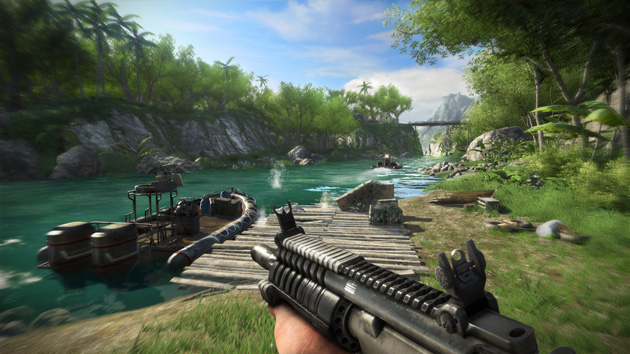
\includegraphics[scale=0.62]{farcry3.jpeg}
	\caption{Far Cry 3 is a RPG featuring an open world}
	\label{fig:farcry3}
\end{figure}

In an open world vehicle simulation videogame, the player would be free to drive around a big city or the long roads of the country side.

\begin{figure}[H]
	\centering
	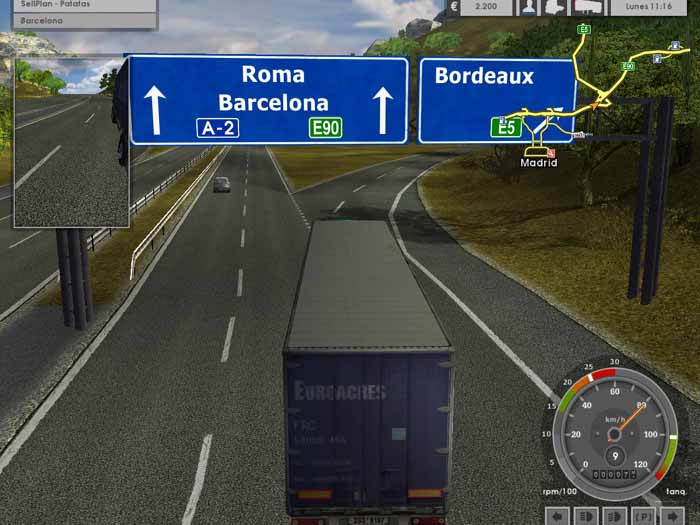
\includegraphics[scale=0.48]{eurotruck.jpg}
	\caption{Euro Truck Simulator is a driving simulator with a realistic open world}
	\label{fig:eurotruck}
\end{figure}

\subsection{Content generation}
\label{sec:contentgen}

Since open world games have such a big universe, there must be a lot of content to fill up all that space. It is required to have a lot of people creating that content (programmers, designers, artists...). Sometimes, when there are not so many human resources available, it is a good choice to generate the world procedurally. Therefore, we can get help from the computers in order to fill the world with fun content. Most of the times, there is a mixture of procedurally generated content and artists content. But there are some games where the content generated by algorithms is predominant. Having the computers to do such a costly task is an advantage for indie game studios because they can not afford hiring so much people. \emph{No Man's Sky}\footnote{\emph{No Man's Sky} is a game produced by \emph{Hello Games}} is an example of a videogame with a procedurally generated world developed by a small team.

\begin{figure}[H]
	\centering
	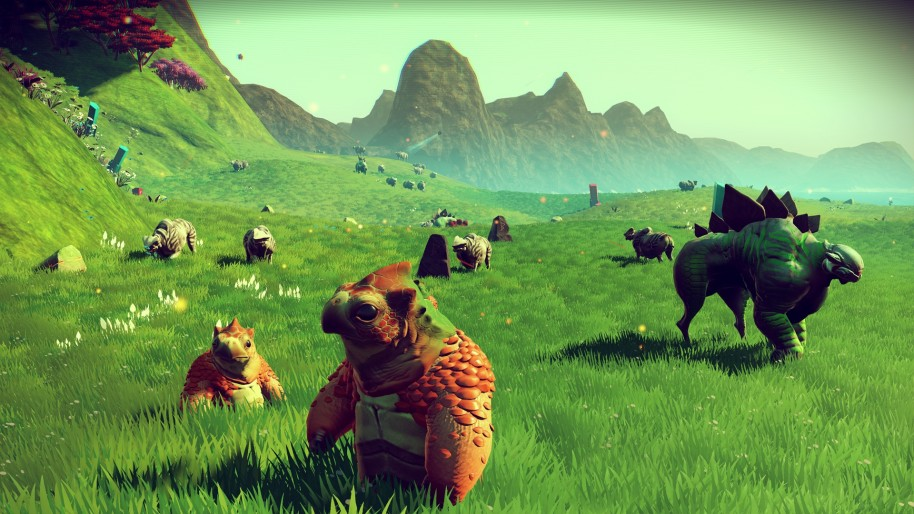
\includegraphics[scale=0.52]{nomanssky.jpg}
	\caption{\emph{No Man's Sky} is a videogame with a potentially unending open world (procedurally generated)}
	\label{fig:nomanssky}
\end{figure}

Whether or not the content of open world games has been generated by a computer or a human, there is a common trend in the latest open world videogames: there are less and less loading screens. The videogame designers are trying to avoid loading screens when possible, so the player doesn't have to wait and has his immersion feeling increased. This is accomplished thanks to a techniche called world streaming. This is the main focus of this document.

\section{Requirements}

So we are willing to make a game engine that supports the development of open world games and avoids loading screens. We are going to focus on the requirements that are more specific for open world games. And requirements that are common for most game engines will be left as secondary requirements.

\subsection{Main requirements}

We consider these requirements are the main target to accomplish.

\begin{itemize}

\item \textbf{Visualization:} We said that requirements that are common for any game engine will be treated as secondary requirements. But this is an exception. It is very important to have some kind of visual feedback. We need visualization to test our system. Also, it is important in order to prove that our engine is working properly. So we need to implement a graphical interface even if it is not very fancy. The graphics will be 2-dimensional.

\item \textbf{Memory management:} If there is one thing that characterizes open world games is that they usually have very big worlds. These worlds have a huge amounts of data (entities, textures, meshes, sound, etc). Some of this games require several tens of gigabytes of compressed data in secondary disk. Obviously, we can not expect our users to have that much RAM capacity. The main challenge will be to keep memory consumption to a minimum while not compromising playability or quality. The trick we are going to use is to load into main memory only the things that are closer to the player. Another thing that we will do is to avoid duplicated resources in RAM. For example, there are is a forest that has many trees that share the same set of textures, we must accomplish that each texture is in RAM at most once.

\item \textbf{Accurate physics simulation:} Again, this is a feature that most game engines incorporate. But it is important as a main requirement because accuracy in open world games carry challenges that must be solved. We will talk about this topic later because it is complex and requires its own space ~(\ref{sec:precission}).

\item \textbf{Easy to use:} It is important that making games with our game engine is as easy as with any of the engines we are used to. If our engine was too difficult to use nobody would use it.

\item \textbf{Testable:} We want to be able to see if our engine is working as expected.

\end{itemize}

\subsection{Secondary Requirements}

These requirements would be great to be implemented for a commercial game engine but not the main target of this academic work.

\begin{itemize}

\item \textbf{Sound:} Every game engine has sound and it is not an issue in open world games.

\item \textbf{Scripting:} We could embed some scripting language as it is done in most game engines.

\item \textbf{Advanced graphics:} They have nothing to do with world streaming.

\item \textbf{Persistency:} It would by great if changes made to the world were persistent.

\item \textbf{Efficiency:} Saving computational resources in world streaming will make them available for other tasks like physics simulation or artificial intelligence.

\end{itemize}



\section{Level-based videogames}


Traditionally games have been structured in levels.
In this kind of games the player must complete the current level to advance to the next one. Once one level is completed that level doesn't need to remain in main memory. Therefore, resources can be deleted.
The mechanics of this type of games allows to manage the resources of the game in an easy and efficient way.

\begin{figure}[H]
	\centering
	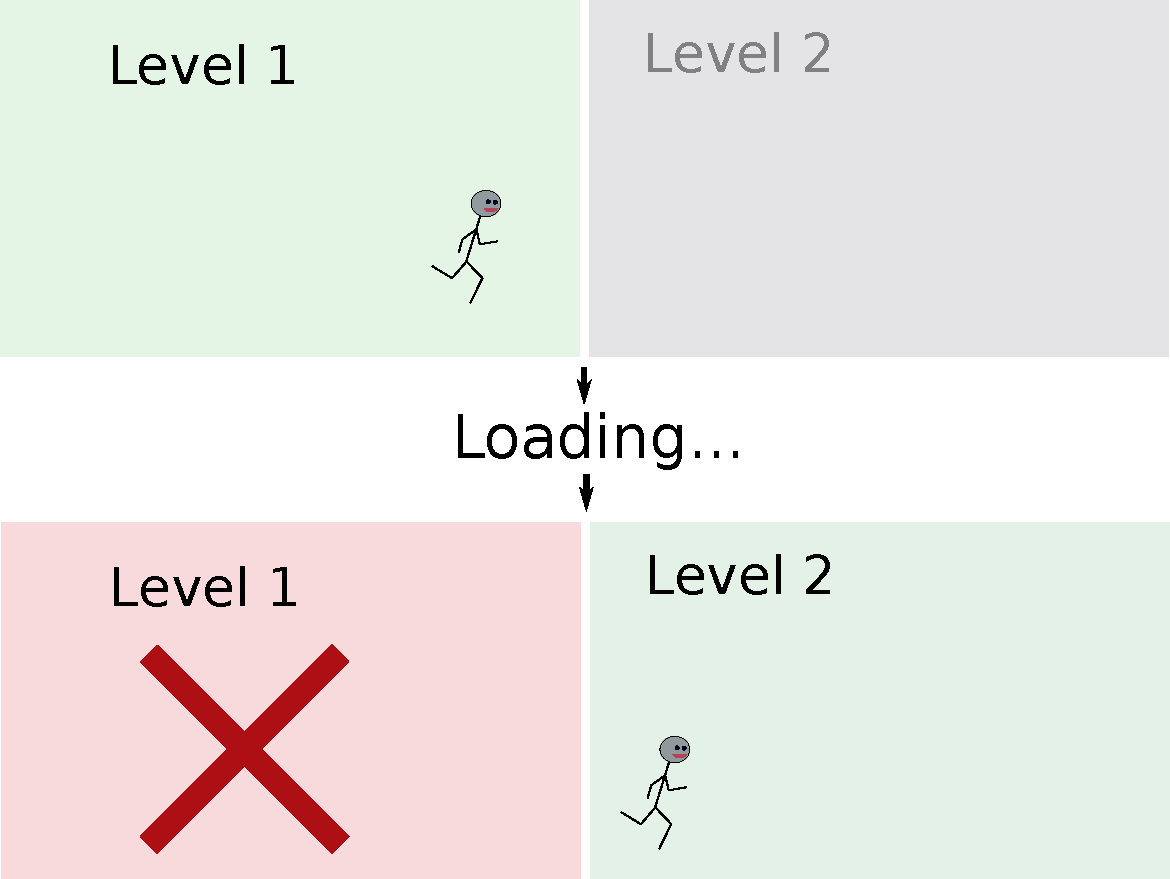
\includegraphics[scale=0.7]{level_loading_mechanics.pdf}
	\caption{Level loading mechanics}
	\label{fig:level_loading_mechanics}
\end{figure}

It is well know that computers(and other gaming devices) usually have two types of memory.
The first memory is the one we usually call main memory. Main memory is fast and small.
The second memory is the secondary storage memory. This one is slow and big. Changing of level requires loading all the resources of the next level from secondary memory and, therefore, it is slow. That's why in most level-based games changing of level will pop-up a loading screen and the player has to wait for a while \cite{levelgame}.

\begin{figure}[H]
	\centering
	
\includegraphics[scale=0.7]{loading_sonic.png}
	\caption{One loading screen from \emph{Sonic}}
	\label{fig:loading_sonic}
\end{figure}

Sometimes, the designers of the game use the loading screen as a mean to give tips to the player.

The approach used by level-based games is not suitable for open world games, we need world streaming in order to avoid loading screens. That doesn't mean there are not open world games that use the level-based approach but, probably, the only reason to implement an open world videogame with loading screens is because it is easier.

\section{World streaming}

World streaming consists on loading game resources and entities on demand. The concept is very similar to video streaming. In video streaming the data is sent from disk or from the network as it is needed. So in world streaming the game contents are taken from the disk (or from the network) to main memory as they are needed.
In contrast to video streaming, world streaming is not as straightforward. In video streaming the data is sequential, that is, you know what comes after. World streaming is different because what comes next depends on what the user does. So we must have the data prepared for all the decisions the user can make.
Imagine the case of a platform game such as \emph{Terraria}\footnote{\emph{Terraria} is a sandbox game by \emph{Re-Logic}}. \emph{Terraria} is a 2D game that has an enormous map.

\begin{figure}[H]
	\centering
	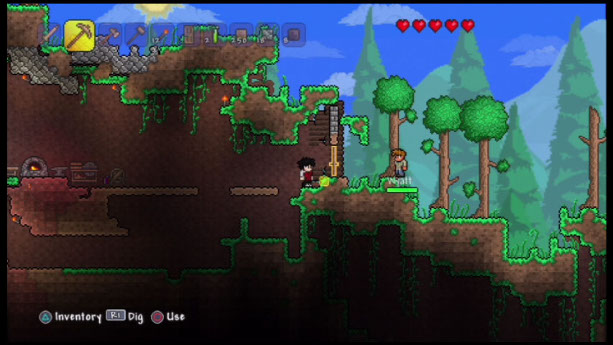
\includegraphics[scale=0.6]{terraria.jpg}
	\caption{Screenshot of \emph{Terraria}}
	\label{fig:terraria}
\end{figure}

In \emph{Terraria} the player can move in four directions (up, down, left, right). So when the user chooses to go to any of the four directions the data must be already prepared in main memory no mater what key is pressed.

\subsection{Examples of games using world streaming}

"Streaming is the backbone of everything we do. Everyone at the company understands how it's structured." said Adam Fowler, the Technical director at Rockstar North \cite{rockstar}.
Companies, such as \emph{Rockstar}, know that world streaming is the technology that supports their success.

In this section we are going to show some of the most relevant games supported by the world streaming technology.

It is pretty easy to find out whether a game is using some kind of world streaming or not. First of all, the game uses less RAM than the size it takes in secondary storage. This would mean that not all the content of the game is loaded at start up (which could be the case in small sized games like Retro City Rampage DX\cite{retrocitysmall}). The second characteristic that identifies games using streaming is the lack of loading screens when moving around (there can be still some loading screens like the first one and when taking portals).

\paragraph{\emph{Hunter} - Paul Holmes (1991)}

\emph{Hunter} is one of the main influences of GTA (\emph{Grand Theft Auto}). \emph{Hunter} is a 3D action-adventure game in which the player could travel around a pretty big world. The degree of freedom in this game was enormous. There were many vehicles (bicycles, cars, ships, tanks, airplanes), places, and weapons. It is certainly not the first open world game but from the information we have I could affirm it might be the first game that used some kind of world streaming.

\begin{figure}[H]
	\centering
	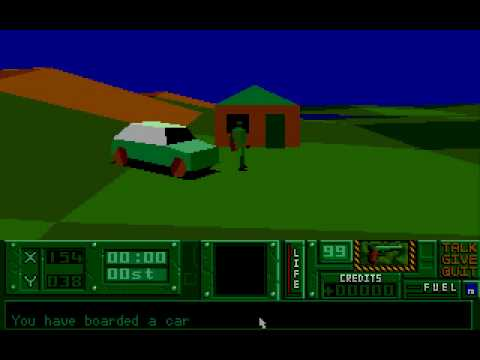
\includegraphics[scale=0.7]{hunter.jpg}
	\caption{Screenshot of \emph{Hunter}}
	\label{fig:hunter}
\end{figure}

In this game there were missions that could be completed but it was the player who decided whether or not to complete them.

Hunter was released for Amiga and Atari. The acceptance of the game was great and magazines ranked it with high scores.


\paragraph{\emph{Grand Theft Auto} - \emph{Tarantula Studios} (1997)}

This was the first \emph{Grand Theft Auto}. With an enormous city and \emph{mainly} 2D graphics, GTA was the one that started the famous series of violent games. The player takes the role of a criminal that can drive all around the city without loading screens.

\begin{figure}[H]
	\centering
	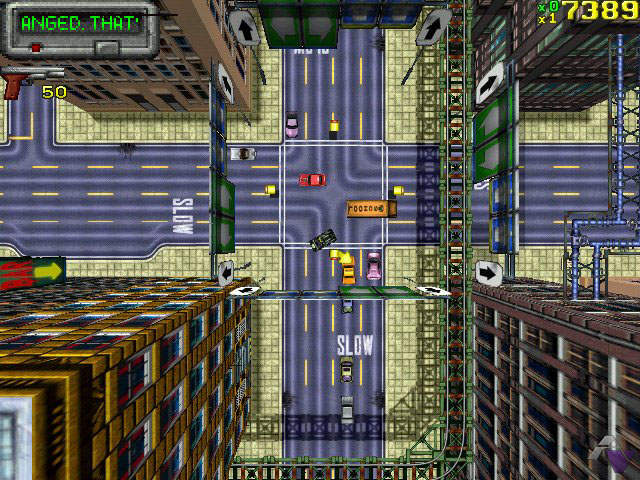
\includegraphics[scale=0.8]{gta.jpg}
	\caption{Screenshot of \emph{GTA}}
	\label{fig:gta}
\end{figure}

The game was released in 1997 for \emph{PC} and \emph{PlayStation}, and in 1998 for \emph{GameBoy Color}. The \emph{GBC} (\emph{GameBoy Color}) version is considered to be a great technological achievement due to the hardware limitations of the portable console. The first \emph{GTA} was successful in sells mainly thanks to the \emph{GBC} version but magazines and users rated it low\cite{gta1}.


\paragraph{\emph{Midnight Club: Street Racing} - \emph{Angel Studios} (2000)}

\emph{Midnight Club} is a series of open world racing games. In this game you take the role of an urban street racer. The player can drive all around \emph{The Big Apple} and challenge other street racers. In the missions you will have to defeat your enemies and scape from the cops. Completing missions will provide you respect and money to buy new cars. But you can skip missions and just enjoy driving around New York.

\begin{figure}[H]
	\centering
	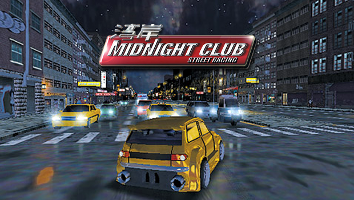
\includegraphics[scale=1]{midnight1.png}
	\caption{Screenshot of \emph{Midnight Club: Street Racing}}
	\label{fig:midnight1}
\end{figure}

This first \emph{Midnight Club} was released in the same year that the \emph{PS2} (\emph{PlayStation 2}) was commercialised. The acceptance of the public was good but sells were less than expected. One year later, they released the \emph{GBA} version which was rated poorly. Despite of its unfortunate sales, this game is the one that started a successful saga.

\paragraph{\emph{Dungeon Siege} - \emph{Gas Powered Games} (2002)}

\emph{Dungeon Siege} is a role-playing videogame very similar to \emph{Diablo} series. Scott Bilas, one of the developers of the game, published a very inspiring article about how the team managed to develop a game with such a big world\cite{worldbilas}. Thanks to its flexible scripting engine the community was able to make modifications of the game, and even some people used the engine to make their own game. Despite the main story of the game is very linear there are many secondary missions and the player has quite freedom to move around. The greatest achievement of this game was avoiding all loading screens except for the initial one. Even taking portals is instantaneous. Graphics were impressive for the time being.

\begin{figure}[H]
	\centering
	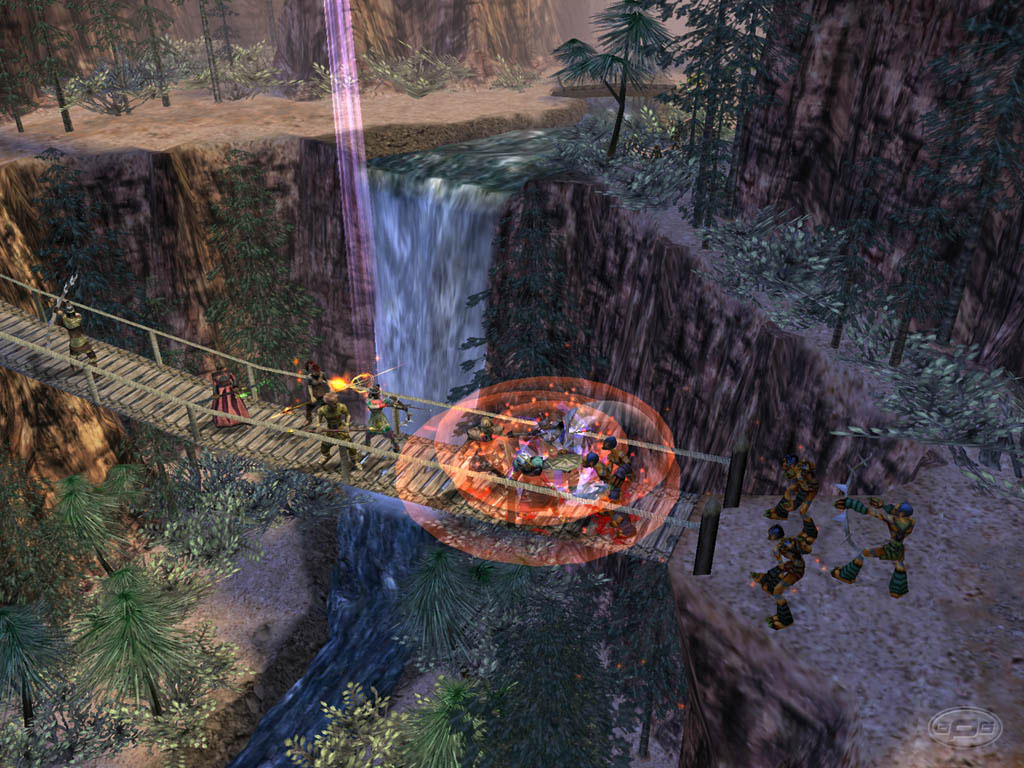
\includegraphics[scale=0.75]{dungeon_siege_screenshot.jpg}
	\caption{Screenshot of \emph{Dungeon Siege}}
	\label{fig:dungeonsiege1}
\end{figure}

\emph{Dungeon Siege} had an online mode too. In the online mode you could grab your friends and complete the adventure in company.

\emph{Dungeon Siege} had good sales but maybe not as much as it deserved for its technological quality and good graphics design

\paragraph{\emph{Grand Theft Auto: San Andreas} - \emph{Rockstar North} (2004)}

After the \emph{Rockstar}'s successful titles \emph{GTA III} and \emph{GTA: Vice City}, it came an even more sold game: \emph{GTA: San Andreas}. Take the role of \emph{Carl Johnson}, the feared gangster. This game has one of the biggest maps in the history of videogames. There is complete freedom to wander around any of the three enormous cities.

\begin{figure}[H]
	\centering
	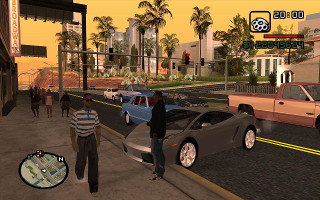
\includegraphics[scale=1]{sanan.jpg}
	\caption{Screenshot of \emph{GTA: San Andreas}}
	\label{fig:sanan}
\end{figure}

\emph{San Andreas} is the most sold \emph{PS2} game ever. Very successful for the \emph{PC} and \emph{XBOX} platforms too. And not only that, the game is still having good sales for \emph{PC} and \emph{Android}.

\paragraph{World Of Warcraft - Blizzard (2004)}

\emph{World of Warcraft} (\emph{WoW}) is an MMORPG (massively multiplayer online role-playing game). This game has a different type of world streaming from the one we have seen so far. In this case the information that provides the status of the entities does not come from the hard disk but from the network. World streaming in the network is even more challenging but, for instance, resource management is very similar. This game has a big world and social interaction between players. Chatting, trading and fighting with other players is possible in \emph{WoW}.


\begin{figure}[H]
	\centering
	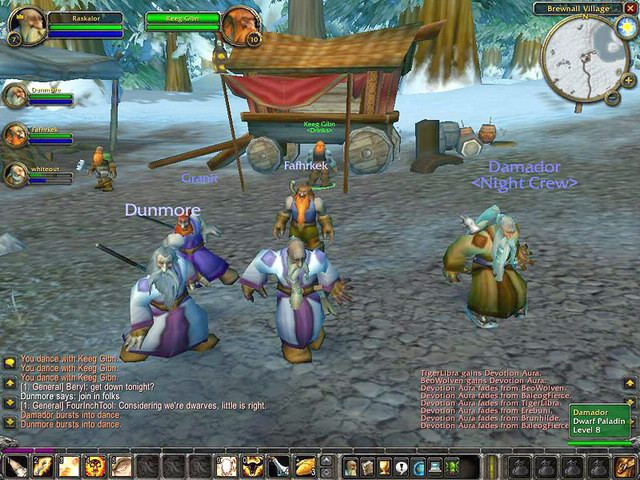
\includegraphics[scale=0.6]{wow.jpg}
	\caption{Screenshot of \emph{World of Warcraft}}
	\label{fig:wow}
\end{figure}

\emph{WoW} has been the most played multiplayer game for many years and it is the game that provided most earnings of all times(\$10 billion)\cite{earnings}.

\paragraph{\emph{Fallout 3} - \emph{Bethesda Softworks} (2008)}

World streaming is a feature present in many of the new-generation videogames. \emph{Fallout 3} is just one of them that has an enormous world and impressive graphics.

\begin{figure}[H]
	\centering
		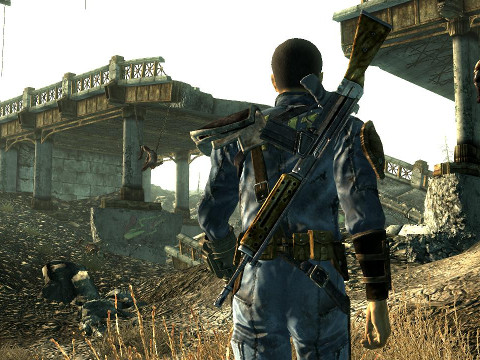
\includegraphics[scale=0.8]{fallout.jpeg}
	\caption{Screenshot of \emph{Fallout 3}}
	\label{fig:fallout}
\end{figure}


\paragraph{\emph{Minecraft} - \emph{Mojang} (2011)}

\emph{Minecraft} is the sandbox that proved that games are not all about graphics.

\begin{figure}[H]
	\centering
	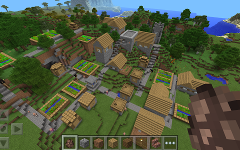
\includegraphics[scale=1]{minecraft.png}
	\caption{Screenshot of \emph{Minecraft}}
	\label{fig:minecraft}
\end{figure}

\emph{Minecraft} is the most sold PC game of all times.


\paragraph{Conclusion}

We have seen many games supported by the world streaming technology. The trend shows that open world games are becoming more popular and it does not seem it is going to stop.

\subsection{The strategy}

The most valuable source of information I have found about world streaming is an article called \emph{The Continuous World of Dungeon Siege} by \emph{Scott Bilas}\cite{worldbilas}. In this article, \emph{Scott Bilas} explains how they developed \emph{Dungeon Siege}. \emph{Dungeon Siege} is an open world 3D game released in 2002. It was developed by \emph{Gas Powered Games} and distributed by \emph{Microsoft}. In this article I have found many useful tips for implementing an open world streaming engine. \emph{Dungeon Siege} is a 3D game but you can only move in four directions (the world is landscape shaped). So the approach followed in \emph{Dungeon Siege} is similar to the one we would follow in a 2D game.

In \emph{Dungeon Siege} the world is divided into pieces of land which are aligned to a grid. These rectangles of land are called nodes. Any node can be connected to every other node. If two nodes are linked, that means that if the player is in one of them, he could travel to the other at any moment. Therefore, when the player is in one node we must be loading at least all the directly connected nodes. Normally the connections will match the adjacent pieces of land.

\begin{figure}[H]
	\centering
	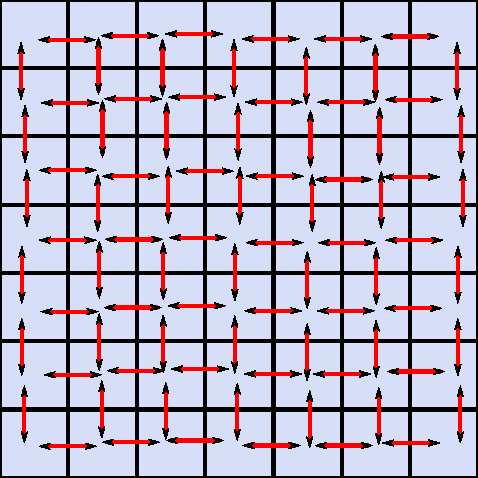
\includegraphics[scale=1]{connections.pdf}
	\caption{Connections of adjacent pieces of land (we are not taking into account the diagonals)}
	\label{fig:connections}
\end{figure}

But there are cases in which two adjacent nodes could not be connected (e.g. there is a wall separating them). Or there could be nodes that are connected and are not adjacent (e.g. there is a portal that will teleport the player from one place to another).


\begin{figure}[H]
	\centering
	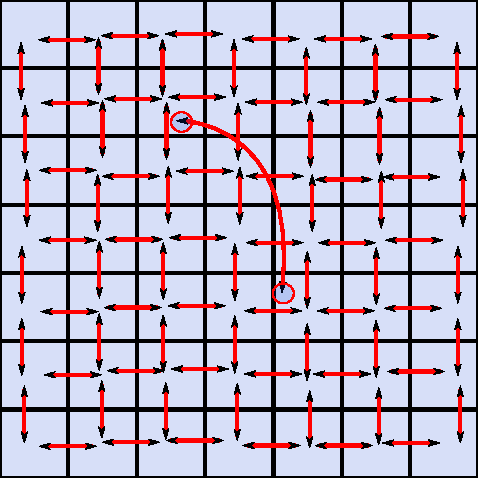
\includegraphics[scale=1]{connections2.pdf}
	\caption{Two nodes connected by a portal.}
	\label{fig:connections2}
\end{figure}

This node-based approach is the one used in \emph{Dungeon siege}. The designers of the game used a custom tool that would allow them to manage the connections of the nodes.

For our engine we are going to take a simpler approach and we will assume each node is connected to all the surrounding nodes (i.e 8 nodes at most). This will simplify the job of the designers of the game. With our approach taking portals will require a loading screen (which is very common current games).

\subsection{Loading Resources is slow}

Imagine that we have implemented our strategy and in a given moment the player has changed of node. We will have to load to main memory all the entities that are located in the new adjacent cells (or nodes). That implies: loading from disk the file that describes that cell, parsing that file in order to find the entities, loading all the resources that are required by the entities and finally creating the entities. So when the node had been loaded you would realize that you have spent 1 second (or much more) and in this time you haven't rendered a single frame!. This would be perceived by the user as a freeze. Therefore, we have to solve this in some way.

\begin{figure}[H]
	\centering
	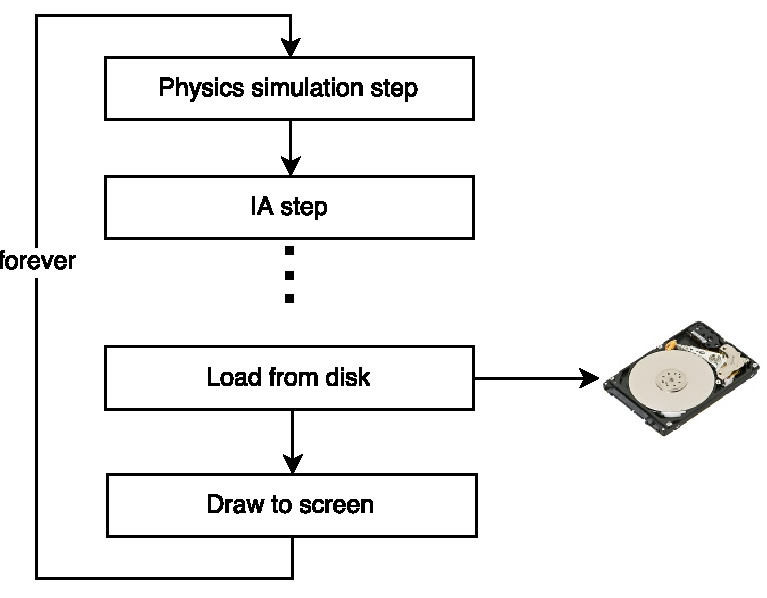
\includegraphics[scale=0.6]{game_loop_disk.pdf}
	\caption{Loading from disk in the main loop.}
	\label{fig:mainloop}
\end{figure}

The bottleneck here is the access to disk. Access to disk blocks the CPU and requires some time. So most of the time, when loading a new cell, the CPU would be idle while it could be doing important tasks (e.g. physics simulation or rendering). The solution that is suggested in the article of \emph{Scott Bilas} (and the one we have followed) is to use a separate thread for loading resources from disk. So if our main thread (the one that executes the main loop) needs to load a resource, instead of doing it itself, it asks the background thread to do it. This way, the main thread is never idle when there is job to be done and the secondary thread will be loading from disk at its own pace.

\begin{figure}[H]
	\centering
	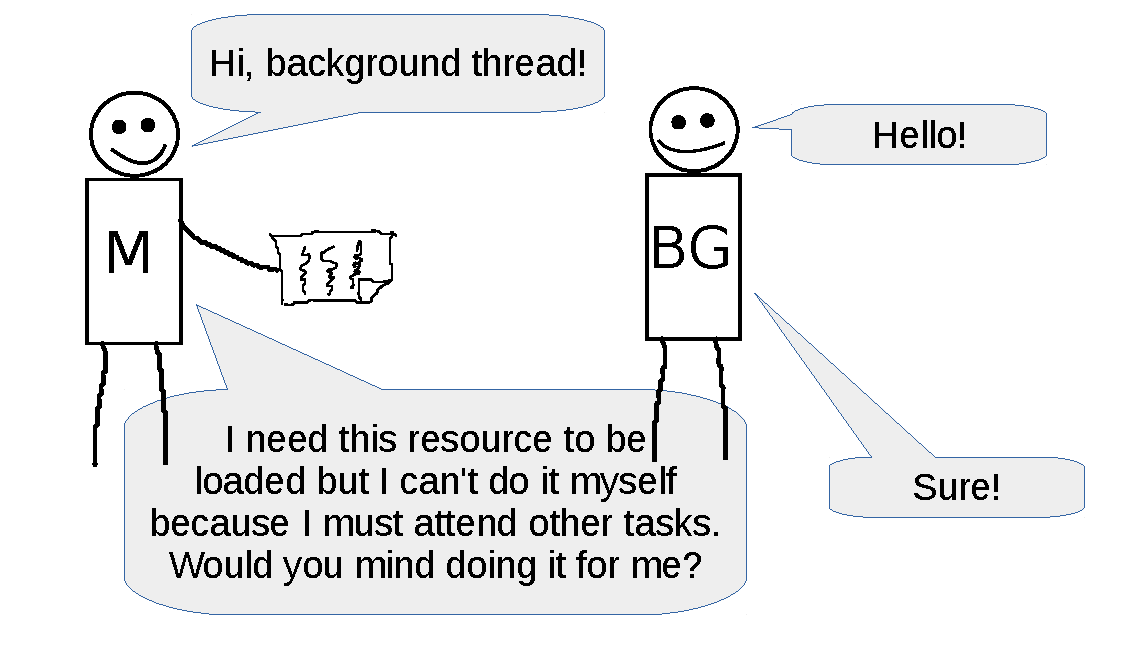
\includegraphics[scale=0.7]{comic1.pdf}
	\caption{Two threads talking.}
	\label{fig:comic1}
\end{figure}

\begin{figure}[H]
	\centering
	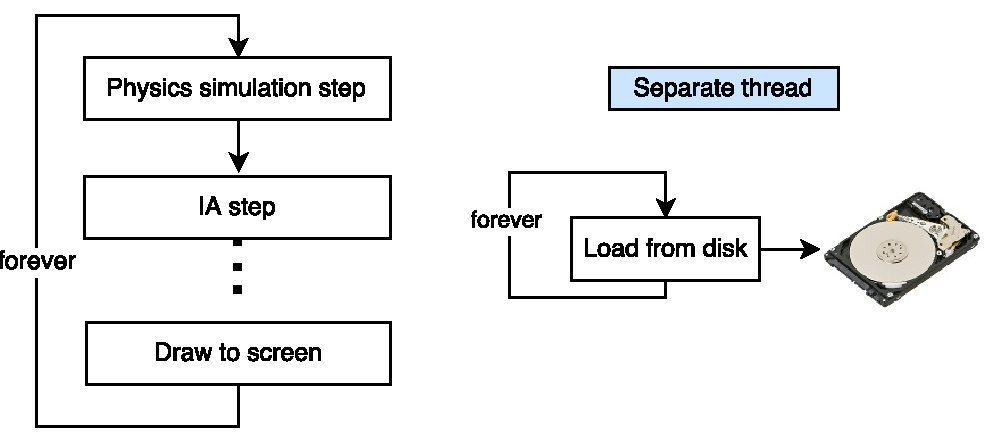
\includegraphics[scale=0.7]{game_loop_disk_2.pdf}
	\caption{Loading from disk is performed by a secondary thread}
	\label{fig:mainloop2}
\end{figure}

\section{The architecture of the engine}

Our game engine will be composed by some subsystems.
In order to work properly the components of the engine must interact with each other in some way.

\begin{figure}[H]
	\centering
	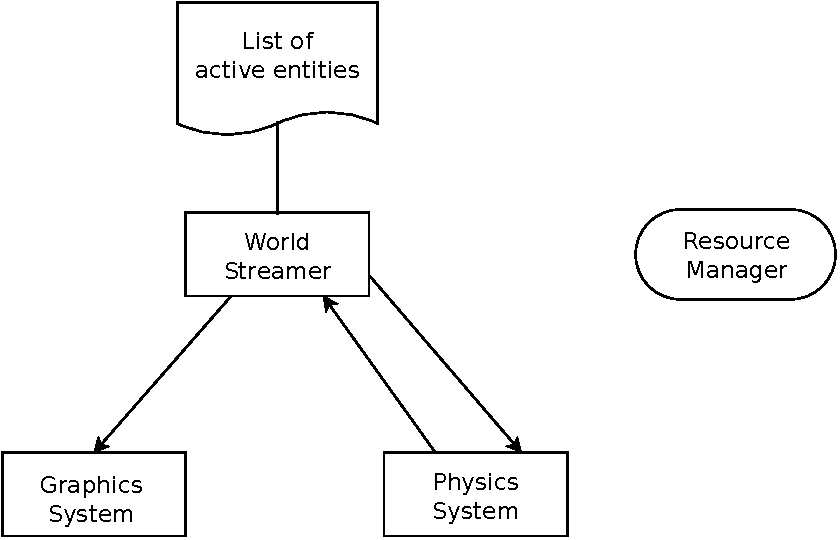
\includegraphics[scale=0.8]{architecture.pdf}
	\caption{Game engine architecture.}
	\label{fig:arch}
\end{figure}

The picture above is a simplification of the architecture. Notice that in the diagram only two subsystems are represented. The graphics and physics components are the most important subsystems, but there could be others like sound or artificial intelligence (AI).

\paragraph{Resource Manager:} The resource manager is the component in charge of accessing the file system. It runs on a separate thread so it does not interfere in the progress of other tasks. Also, it must assure that there will not be duplicated resources in main memory. The resource manager is used by all the other architecture components. So it takes the role of a servant for the others. In other to ease the access to this utility system, it is very convenient to implement it as a singleton.

\paragraph{World Streamer:} It is the one. The brain of the architecture. The world streamer is in charge of telling the subsystems below (graphics and physics in our diagram) what to do. It must decide whether a given entity must be loaded or not. An inefficient implementation of the world streamer would decide that all the entities of the world must be loaded. And a useless implementation would not load any entity. So the world streamer needs to compute the subset of entities that must be loaded at any time. This subset of loaded entities is what we find in the diagram as "List of active entities".

\paragraph{Graphics System:} Might be called graphics engine too. It will get a list of entities that must be rendered from the world streamer. So it will be just told what should be displayed on the screen. The graphics system is independent from all the other components and does not care who is using it.

\paragraph{Physics System} Very similar to the graphics system. In the diagram you can appreciate the difference between these two: an extra arrow. This arrow flows from the physics system to to the world streamer. The meaning of this arrow is the position of the main character. After each physics simulation step the position of the main character might have changed and the world streamer needs this information in order to recompute the set of active entities.

\section{Implementation}

In this section I will explain briefly how I implemented the modules of the game engine.

\subsection{Graphics System}

The graphics system is implemented from scratch (there is a reason that will be explained later). Since implementing a graphics engine is not the purpose of this academic work, it does not have a big set of features.

\subsubsection{Architecture}
This graphics module is split in two layers. The first layer is the low-level layer. The low-level layer is the one that uses the OpenGL API (application programming interface). The purpose of the low-level layer is to provide a simple interface for the upper layer. This way the high-level layer does not need to understand any of OpenGL. So if we needed to deploy the application to a platform were DirectX performs better, we would only need to replace the low-level layer and the rest of the whole system would remain the same.

\begin{figure}[H]
	\centering
	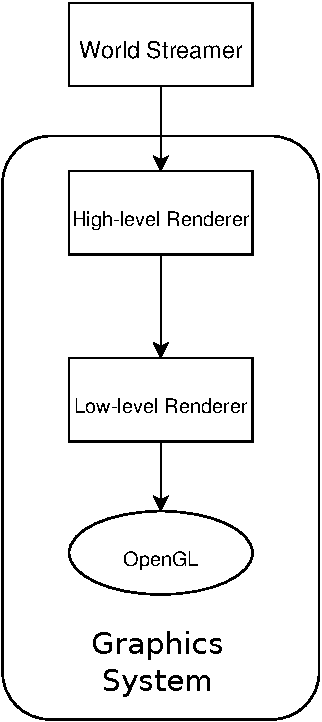
\includegraphics[scale=0.8]{renderer.pdf}
	\caption{Graphics system architecture.}
	\label{fig:renderer}
\end{figure}

The low-level renderer API is just a reduced set of functions that allows to draw things on the screen. On the other hand the high-level renderer provides a class-based mechanism to define the scene. That is, in the low-level renderer we would say: "draw texture A in position X" and it will be shown on the screen for just this frame. And in the high-level renderer we would say: "there exists a sprite in X and it has priority P" and it would be drawn on the screen until it is removed.

\subsubsection{Features}
The renderer I have implemented is not very sophisticated but works fine for our purpose. Animations are not yet supported(Update: I have implemented a new animation system [\ref{"sec:animationsystem"}]). You can assign priorities to the sprites in order to define what is drawn on top. There is an abstraction of the camera too. The low-level renderer uses the subset of functions available in OpenGL ES (embedded systems), so it could be ported to mobile platforms.

\subsubsection{Why did I implement my own graphics engine?}

There are three reasons I had to implement a custom graphics engine.

\paragraph{Most graphics engines will manage resources automatically.}
Automatic resource management is one of the main targets of this academic work. If we had the render engine to do this for us, we would be missing something important. Even though, the graphics engines only manage graphics related resources and we would like to have resource management unified. What is more important, the resource manager of the graphics engines might be blocking.

\paragraph{OpenGL implementations do not support multithreading.}

OpenGL does not allow you to call its functions from threads other than the main thread. If you try to do so the behavior will be completely undefined \cite{multiopengl}.

Loading a graphics resource (like a texture) involves these steps:
\begin{itemize}

\item \textbf{Load the resource, which is stored in hard disk, to main memory.} This must be done by the secondary thread because we are accessing hard disk and that is slow.

\item \textbf{Allocate the resource in video card memory.} To render an object all its resources must be in the memory of the graphics card. To allocate, for instance, a texture in video memory we need to call OpenGL functions. That is the reason this step must be performed by the main thread (only the main thread is allowed to call OpenGL functions). Fortunately, the process copying a resource from RAM to VRAM is fast enough, so it does not block other tasks.

\item \textbf{Delete the resource in MM.} Once the resource is in VRAM, we do not need it anymore in RAM. This task is not costly and could be performed by any thread. In our implementation it is deleted by the secondary thread because we think it makes more sense that the memory is released by the same thread it was allocated by. Also, in this way the code seems better encapsulated.

\end{itemize}

Most graphics engines provide functions to load graphics resources. And these functions do all the steps that we mentioned in a single call. Therefore, if we used one of these graphics engines, we would not be able to split the work among the two threads. Probably, there are workarounds that would allow to split tasks but they might difficult to implement. This is the main reason I have decided to make my own render engine.

\paragraph{I had personal interest in learning modern OpenGL.}

Also, I wanted an excuse to learn modern OpenGL features like shaders. The version of OpenGL I used is OpenGL ES 2.0. This version of OpenGL is compatible with embedded systems, smartphones and tablets. In this version you are forced to use shaders because all the fixed pipeline functionality has been removed. I will dedicate a section to explain briefly how to use shaders in modern OpenGL.

\subsubsection{Modern OpenGL programming}

I do not pretend to make a tutorial on modern OpenGL nor shaders but just to summarize what I have done.
I have used only the subset of API that is common to OpenGL 2.1 and OpenGL ES 2.0. In my testings, I used version 2.1, which is the one that runs on PC.

Since OpenGL ES does not support fixed pipeline functions I had to use shaders. What are shaders? Basically , they are pieces of code that run in the graphics card. They are used to achieve custom visual effects\cite{shader}. In OpenGL shaders are written in a specific programming language called GLSL. GLSL is very similar to C\cite{glsl}].

There are two types of shader.

\begin{itemize}

\item \textbf{Vertex shader.} Vertex shaders take as input one vertex and gives as output the position (or other properties like normal and UV coordinates) that vertex should take. It is used to achieve effects such as mesh deformation. One example where vertex shaders are used is the waves of the ocean. The vertex shader should change the position of vertices  so it fakes the water moving. In our 2D render engine, we do not need the vertex shader to do anything special: it just forwards the position as it is.

\begin{minted}{c}

#version 120

/**
 * In the vertex shader you are computing the position
 * of the current vertex.
 * Also you compute the texture coordinate corresponding
 * to this vertex.
 **/

// these are the parameters received by the main program
attribute vec2 inPosition;
attribute vec2 inTexCoords;

void main()
{
	
	// compute the position of the current vertex
	// In this case you are just forwarding the position,
	// but this allows you to achieva cool effects like the
	// mesh bending or the waves of the ocean
	// The fouth coordinate is called W(1.0) and it is used
	// for normalization purposes( read: 
	// "http://stackoverflow.com/questions/2422750/
	// in-opengl-vertex-shaders-what-is-w-and-why-do-i-divide-by-it" )
    gl_Position = vec4(inPosition, 0.0, 1.0);
    
    // compute the texture coordina corresponding to this
    // vertex
    gl_TexCoord[0] = vec4(inTexCoords, 0, 0);
    
}


\end{minted}

\item \textbf{Fragment shader.} Also called pixel shader but this term is more used for DierectX. Fragment shader is executed for every pixel and it should output the desired color for the current pixel. In our code we will be returning the color of the corresponding texture coordinate.

\begin{minted}{c}

#version 120

/**
 * In the fragment shader you are computing
 * which should be the color of the current pixel
 * ( fragment and pixel are sinonyms in OpenGL,
 * in fact in DirectX it is called pixel shader )
 * 
 * The output goes to -> gl_FragColor
 * 
 **/

uniform sampler2D tex;

void main()
{
	
	// take the color of the texture pixel
	vec4 color = texture2D(tex, gl_TexCoord[0].st);
	
	// output
    gl_FragColor = color;
    
}

\end{minted}


\end{itemize} 
  

Shaders are compiled at runtime. In the following picture there is a summary of the steps that are required to make a shader program.

\begin{figure}[H]
	\centering
	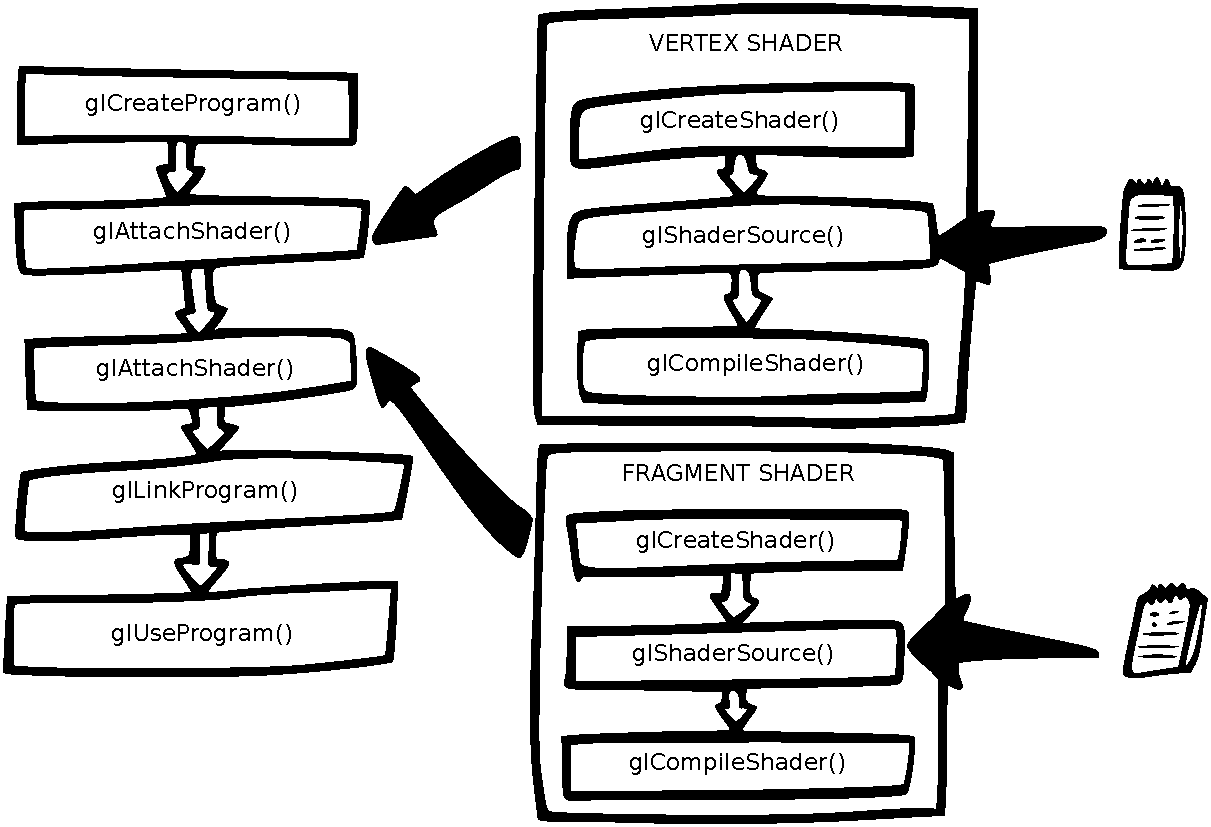
\includegraphics[scale=0.75]{shad.pdf}
	\caption{The process to compile and use shaders.}
	\label{fig:shad}
\end{figure}

Once you have built your shader program you can use it at any time. These are the tutorials that I have learned from: \cite{shadtut} \cite{glmodtut} \cite{learngl}.

Since in modern OpenGL ES matrix operations (such as \emph{glRotatef()}) have been removed I had to use one geometry library: GLM\cite{glm}. For window management I used SDL2\cite{glm}. And for texture loading I employed SOIL\cite{soil}.

\subsection{Physics System}

The physics system we have implemented is not very complex. We have made a small wrapper of Box2D. Box2D is a popular 2D physics engine\cite{box2d}. It is used by, the well known game engine, Unity.

\begin{figure}[H]
	\centering
	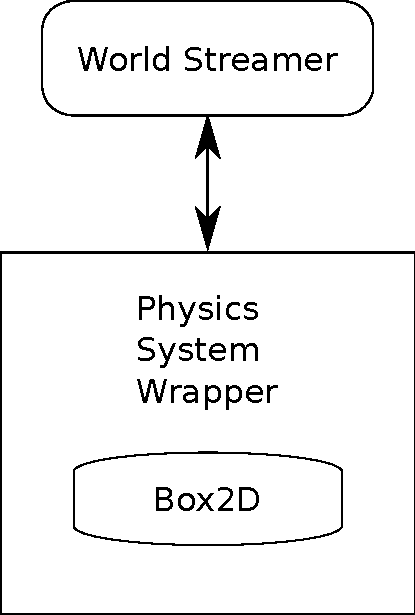
\includegraphics[scale=0.65]{physics_wrapper.pdf}
	\caption{Physics System Architecture.}
	\label{fig:physics_wrapper}
\end{figure}


Our wrapper consists of two main classes: PhysicsComponent and PhysicsSystem. The first one is an abstract class that represents a rigid body. In our engine entities are composed of components and PhysicsComponent is one of them. An entity could have a PhysicsComponent or not.

There are only two implementations of PhysicsComponent: PhysicsBox and PhysicsCircle. PhysicsBox is defined by some and width and height (axially aligned) and PhysicsCircle by the radius. You can assign mass, dimensions and position to it. Also you can chose at creation time if it is dynamic or kinematic. Kinematic bodies will not be affected by forces. Also, if mass 0 is assigned to a body it will be assumed to be static (can't be moved at all).

PhysicsComponent's are created by a request to the PhysicsSystem. When you are done with a PhysicsComponets request its deletion to the PhysicsSystem. The GraphicsSystem and the PhysicsSystem run at the same rate. So in the main loop you only have to call the update function of the two systems.

\subsubsection{The issue of the precission}
\label{sec:precission}

In the requirements section we stated that physics simulation was a main requirement because it was a challenge in big world games. Here it comes the reason. Floating point numbers can be imprecise when they become too high (or too low).

\begin{figure}[H]
	\centering
	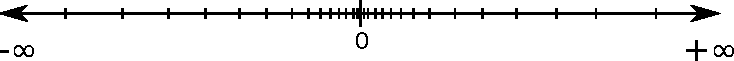
\includegraphics[scale=1]{float.pdf}
	\caption{Float sampling representation.}
	\label{fig:float}
\end{figure}

As you can see, floating point numbers are not distributed uniformly. The sampling rate is better for values that are closer to 0. And the number of represented values decreases as we go towards $-\infty$ or $+\infty$. So in our game the precision would decrease as we get further from the origin of coordinates. That affects mainly the physics simulation but also graphical representation. And this problem becomes worse if the world is very big.

So how can we solve this? Well, if the problem raises because the entities are too far from the origin of coordinates, let us move the entities to where the origin of coordinates is (or move the origin of coordinates to where the entities are). We will retake this topic in the "World streamer" section (\ref{sec:worldstreamer}).

\subsubsection{Alternative approaches}
There are other approaches to overcome the precision issue.

\begin{itemize}

\item \textbf{Using \emph{double}:} Double precision floating point numbers have a broader range and better accuracy. It would be pretty straightforward to replace \emph{float}s by \emph{double}s. But this is not scalable. What if we need even more accuracy?. Also, some graphics cards might not support \emph{double}s. Therefore, animations and visual feedback would look poor.

\item \textbf{Using fixed-point:} Fixed-point numbers (FPN) have constant precision in all ranges. The range might be too small but we can always use \emph{long} integers for a broader range and better accuracy. We could use libraries for even greater integers (BigInt), although this would decrease performance. There are drawbacks for this solution. The physics engine might not support FPNs, eventhough we could spend time modifying the source if it is available. The graphics card might not support them (specially with 64-bit). In genaral, since floating point numbers are so extended, it would be difficult to integrate with existing software.

\end{itemize}

\subsubsection{Our approach}

The approach we have chosen has many benefits and the only drawback is that it is a bit diffucult to implement.

Having the origin of coordinates close to the entities allows us to use the most precise range of floating point numbers. In that range, floating-point is even more accurate than fixed-point.

Since we are using the floating-point numbers that most graphics cards are optimized for, we get the best possible performance. And the compatibility is also the best.

We can use any existing software because floating-point is so extended.

When storing entities for persistence, the positions will be relative to the cell they belong to. So any position in the world could be represented as a pair of cell (integer vector) and relative position (float vector). So as long as the cell size keeps small, the precision will be fine. And the integer representation is broad enough for most cases. If 32-bit integers were not enough, you could always use 64-bit or even libraries such as TTMath\cite{workqueue}. With our representation we have good accuracy and unlimited range scalability without droping performance.

The representation that we have used is the same that Scott Bilas suggests\cite{worldbilas}.

\subsection{Resource Manager}

The resource manager is the system that takes care of accessing the secondary storage memory. It provides all the other system components an interface to get resources when they need them without having to wait.
So basically, the resource manger returns a handle to the resource when it gets a request. Even if the resource is not loaded, it should return a handle (instantaneously).

The following comic shows in a friendly way how the resource manager works.

\begin{figure}[H]
	\centering
	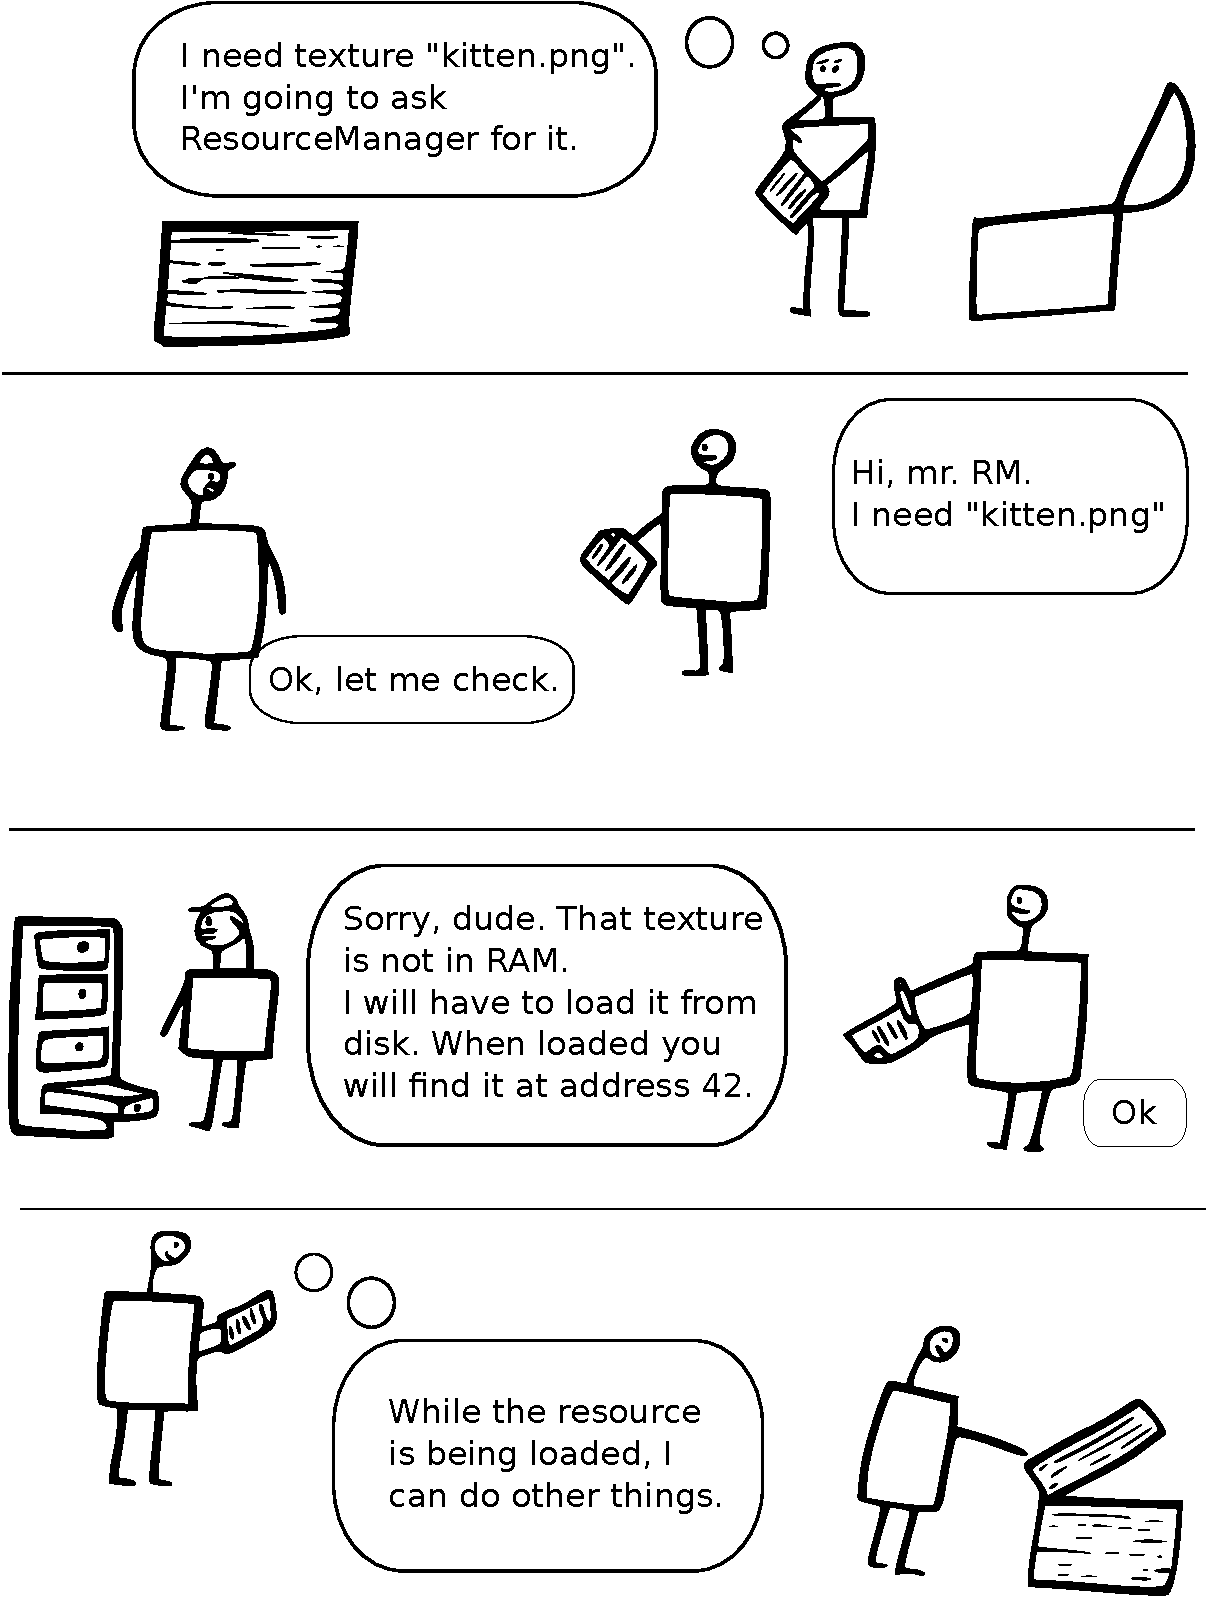
\includegraphics[scale=0.75]{resmancomic.pdf}
	\caption{Comic of the resource manager.}
	\label{fig:resmancomic}
\end{figure}

As you can see, even though the resource manager says that the requested resource is not in RAM, he tells the requester that when it becomes loaded, he will find it at address 42 (that is the handle).

Take a look at (this time more serious) representation.

\begin{figure}[H]
	\centering
	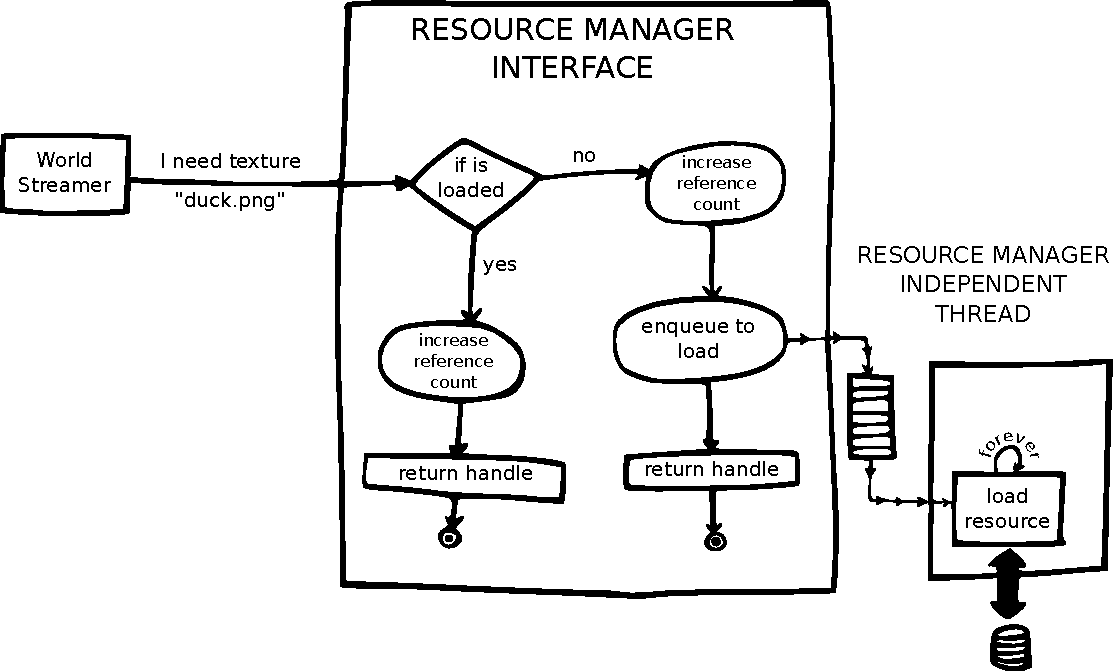
\includegraphics[scale=0.8]{resman.pdf}
	\caption{Diagram of the resource manager.}
	\label{fig:resman}
\end{figure}

The resource handle is returned in all cases. The handle has an attribute that tells if the resource is loaded or not.

So for instance, the renderer needs to draw a texture. Therefore, the graphics system requests to the resource manager that texture. Every frame, the graphics system will check if the resource has been loaded. And if it is, the texture is drawn.

The resource manager needs to keep track of how many handles are pointing to each resource. When the number of handles for one resource becomes zero, the resource is released.

If one resource needs to be loaded, that request is enqueued in a special queue. What is so special about this queue is that it is prepared for being accessed by several threads (thread safe queue). This type of queue is usually called work queue.

In our implementation there is the abstract class Resource. These are some of the classes that inherit from Resource:

\begin{itemize}

\item{\emph{\textbf{ResourceText}}}. It represents a text file on disk. When loaded you will be able to read the file using "\emph{getText()}".

\item{\emph{\textbf{ResourceTexture}}}. This is the resource that will be required by the sprites. When loaded you can call "\emph{getTextureData()}" and you will be given a pointer to the raw texture data.

\item{\emph{\textbf{ResourceCell}}}. This resource is quite special. When loaded, you will be able to get the data also. But this time you can modify the data. You are given a XML node and you can modify it. When there are no references to a \emph{ResourceCell} it will be released and all changes made will be stored. This resource is used to represent a cell where entities can be placed. Therefore, you can add and remove entities from the cell and seamlessly all changes will be persistent.

\end{itemize}

The resource manager is a singleton and needs to be initialized at the beginning of the application. In order to do so, just call "launch()". That will start the secondary thread.

In order to implement the work queue, I used pthreads and I got inspired by this article\cite{workqueue}.

\subsection{World Streamer}
\label{sec:worldstreamer}

The world streamer is in charge of telling which entities should be loaded and which ones should be deleted. The world is divided in equally sized squares and inside each of these cells we will place the entities.

\begin{figure}[H]
	\centering
	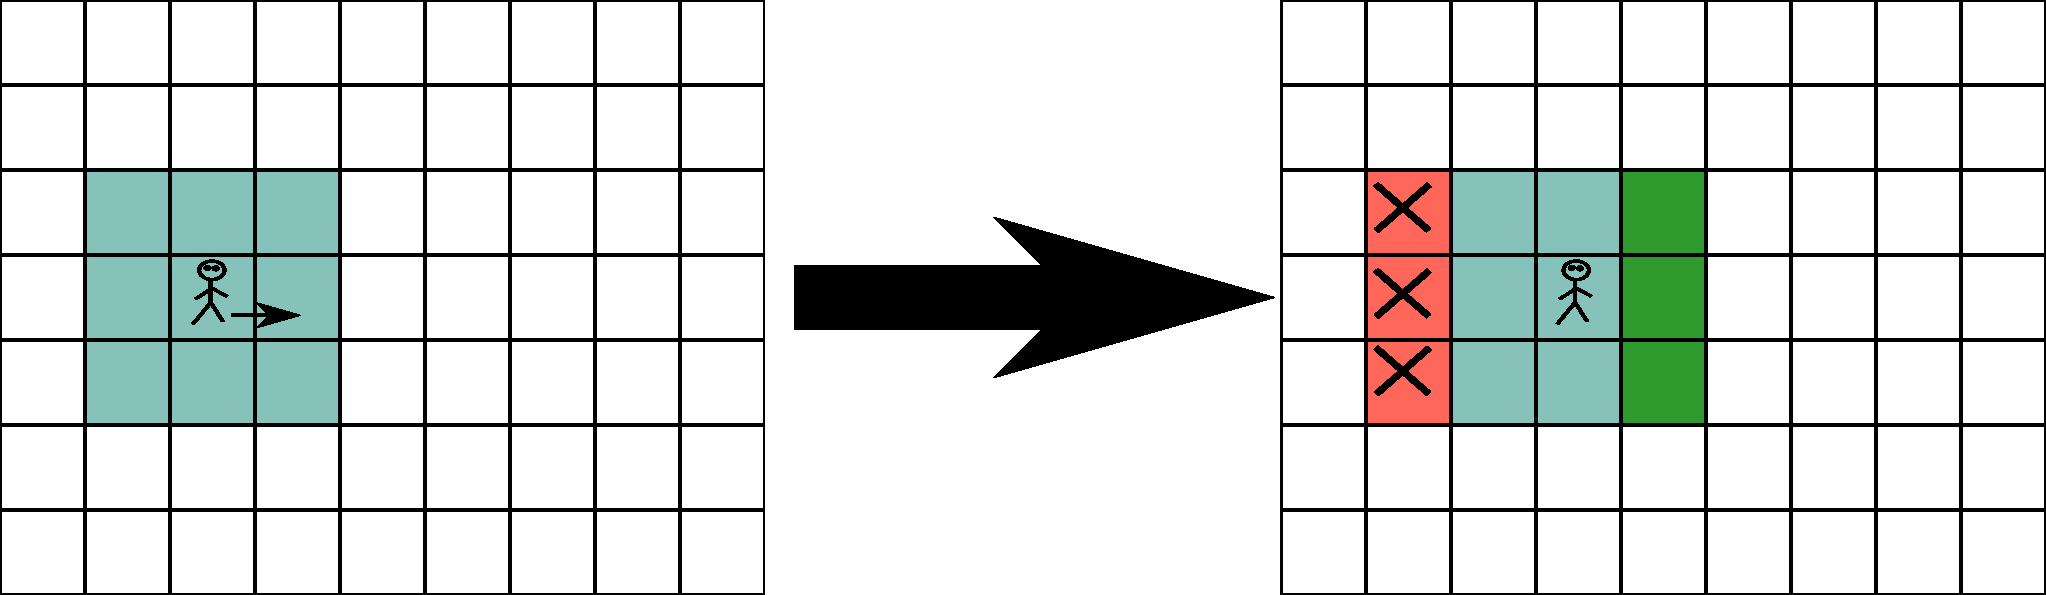
\includegraphics[scale=0.35]{grid.pdf}
	\caption{When changing of cell some cells are loaded and some others become deleted.}
	\label{fig:grid}
\end{figure}

Each cell is represented in an XML file and they are named as "cell\_X\_Y.xml".
Take a look at this example of XML file:

\begin{minted}{xml}

<cell>
	<entity>
		<position>
			<x>109.925</x>
			<y>180.015</y>
		</position>
		<graphics>
			<texture>tukifoc.png</texture>
			<width>120</width>
			<height>120</height>
		</graphics>
		<physics>
			<shape>box</shape>
			<width>120</width>
			<height>120</height>
			<mass>60</mass>
		</physics>
	</entity>
	<entity>
		<position>
			<x>9.91001</x>
			<y>112.793</y>
		</position>
		<graphics>
			<texture>wood_box.png</texture>
			<width>80</width>
			<height>80</height>
		</graphics>
		<physics>
			<shape>box</shape>
			<width>80</width>
			<height>80</height>
			<mass>60</mass>
		</physics>
	</entity>
</cell>

\end{minted}

In this example you can see there are two entities attached to the root node (cell). Each entity has position, graphics component and physics component. Inside the graphics component there is the texture and the dimensions. In some cases, you will find "priority" for the graphics component. If the priority is not specified, zero will be assumed.

At he beginning the world streamer will search in the "world\_folder" directory for all files named like "cell\_X\_Y.xml" (where X and Y are integers). The are no restrictions in the shape of the world. All the following shapes are valid.

\begin{figure}[H]
	\centering
	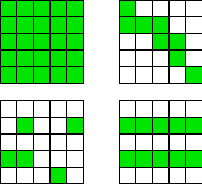
\includegraphics[scale=1]{validworlds.pdf}
	\caption{Examples of valid world shapes.}
	\label{fig:validworlds}
\end{figure}

If an entity gets out of a cell and gets in a space where there is no cell (what is not green in the previous picture), the entity is stored in the last valid cell it was. So it is the job of the designer to make sure no entity will get outside of the map.

\begin{figure}[H]
	\centering
	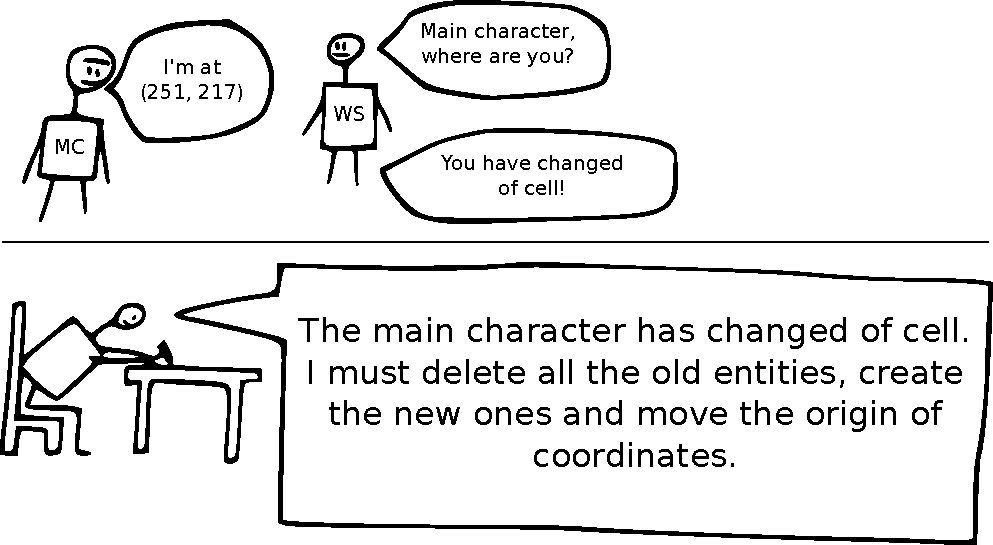
\includegraphics[scale=0.85]{comic2.pdf}
	\caption{World streamer realizes that the main character has changed of cell.}
	\label{fig:comic2}
\end{figure}

The world streamer implements the \emph{IWorldStreamer} interface, so you can have several implementations for the world streamer. In the early beginning, when the \emph{WorldStreamer} was not still implemented, we wrote \emph{TestWorldStreamer}. This class just streams one entity and its implementation was pretty strightforward. This way of programming allowed us to make a fast prototype and check that all the system components were interacting properly. The main functions of this interface are: \emph{init()}, \emph{update()} and \emph{getEntities()}.

The implementation of the \emph{update()} function is the core of the system. It determines the list of active entities. Its implementation is one of the longest but it is not as difficult as it might seem at first. The following diagram sums up what this function does.


\begin{figure}[H]
	\centering
	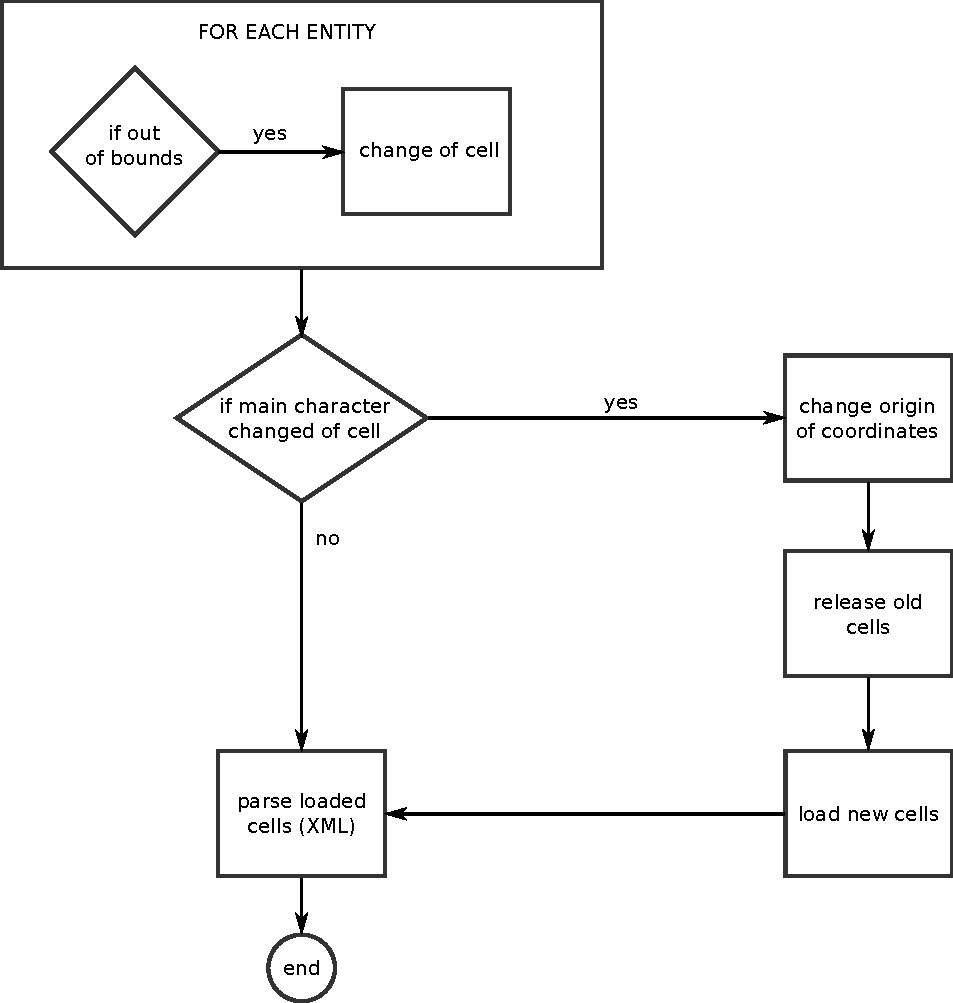
\includegraphics[scale=0.8]{worldstreamer.pdf}
	\caption{Flow diagram of the update function of the WorldStreamer.}
	\label{fig:worldstreamer}
\end{figure}

In each frame we check for cells (XML files) that have been loaded and we parse them. After parsing, we create the new entities.

Deleting a cell involves creating an XML tree, removing all entities and finally requesting the resource manager to release the XML file (thus saving it).

Also, we must handle when the user closes the application. So when the user closes the window or presses \emph{Esc} we must save all the active cells.

In order to parse XML and modify the trees, we have used RapidXml. This library claims to be the fastest out there. There is also a high-level wrapper of this library in the famous Boost library collection but I realized later. Anyhow, I have found it to be pleasant to use. The only pitfall I have found with this library is a small compiling error there is when generating the text of the tree. I seems to be a bug that can be easily solved\cite{rapidxmlbug}.

When I had to implement the code that looks cell files in a certain directory, I had to use a external library: Boost Filesystem. I decided to use this library because of its good portability. Also the Boost libraries are guarantee of quality.

\section{Result and testing}

The final application consists of a stable game engine. Yet not fully-featured.

\textbf{Note:} There is section \ref{"sec:animationsystem"}, where we show a newer version of the engine.

\begin{figure}[H]
	\centering
	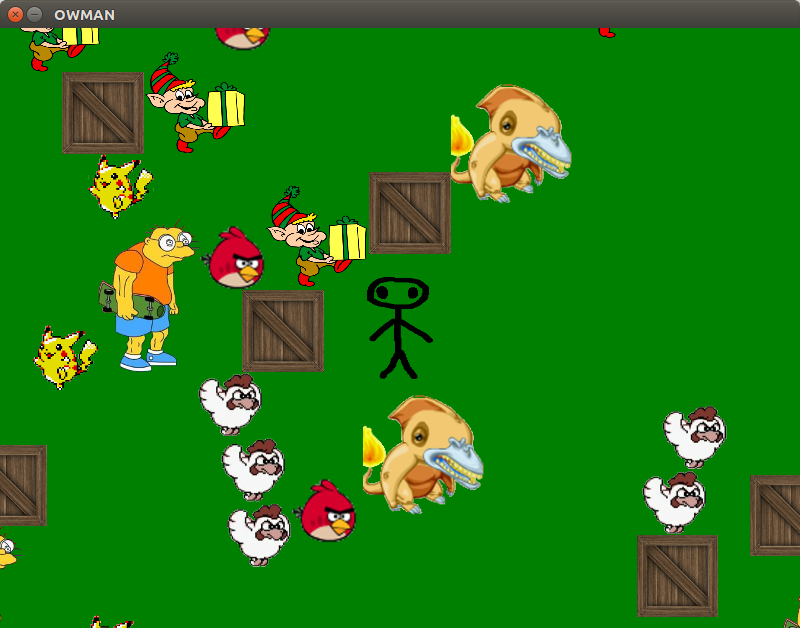
\includegraphics[scale=0.36]{screenshot1.png}
	\caption{Demo screenshot.}
	\label{fig:screenshot1}
\end{figure}

\subsection{Demo}

As you can see, we have developed a demo using our game engine. After a lot of debugging, everything seems to work very well. Graphics are fine, physics are accurate and overall performance is petty good.

In order to test our system intensively, we have written an script that generates a random world. We have made our tests with a world of 1 million cells (which is about 4GB of XML files). The files must be located in the "\emph{world\_folder}" directory. In the same folder there is the main character file (\emph{main\_character.xml}). In this file you can configure the appearance, position and other stuff of the main character.

Our application allows to zoom in and zoom out the camera using the mouse wheel. When you open the application you will see something like in figure \ref{fig:screenshot1}.

If you zoom out the camera you will be able to see the boundaries of the visualization.

\begin{figure}[H]
	\centering
	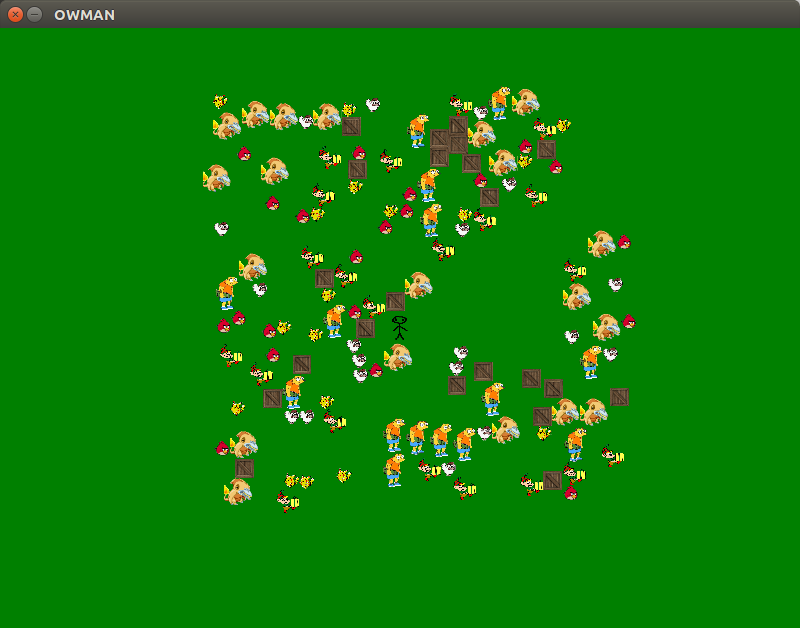
\includegraphics[scale=0.45]{screenshot2.png}
	\caption{Zooming out.}
	\label{fig:screenshot2}
\end{figure}


So if you zoom in enough, the player will not realize that the entities are being loaded a he walks.

You can watch this video of the demo  \url{https://youtu.be/ymecWxF886U}.
The previous video shows the demo at the time the first performance tests where made.

There it is a video of the engine with the latest features (much better looking) \url{https://vimeo.com/159836286}.

\subsection{Performance}

The memory consumption is very low. Running with one million of cells we get a RAM consumption of $\sim$70MB.

The world window is the space that will determine the set of entities that are loaded at any given time. We can configure the size of the world window in \emph{init\_file.xml}. The world window is always square shaped and the side is always odd. The number you have to put in the configuration file is not the side of the world window, it is $(side-1)/2$. This way, the introduced number is always valid.

The following pictures show different world window sizes.

\begin{figure}[H]
	\centering
	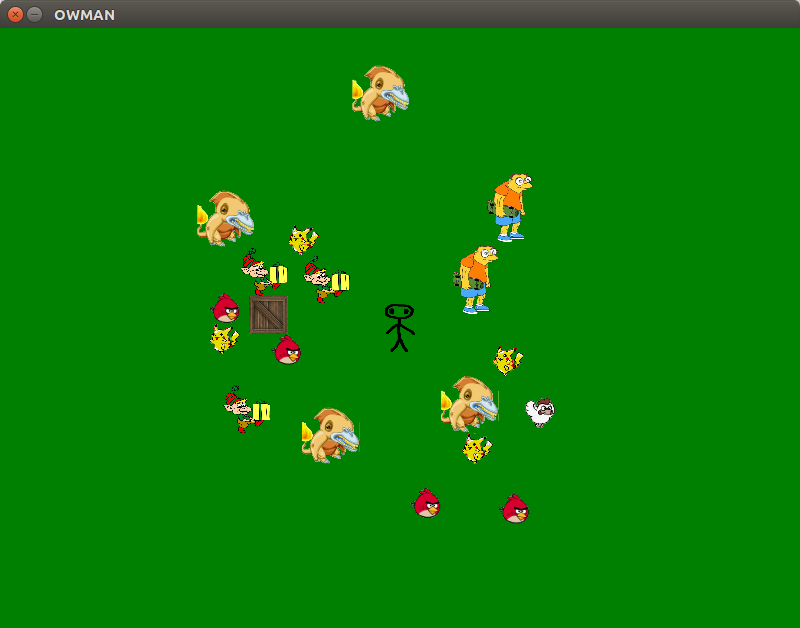
\includegraphics[scale=0.40]{size1.png}
	\caption{Window size = 1.}
	\label{fig:windowsize1}
\end{figure}

\begin{figure}[H]
	\centering
	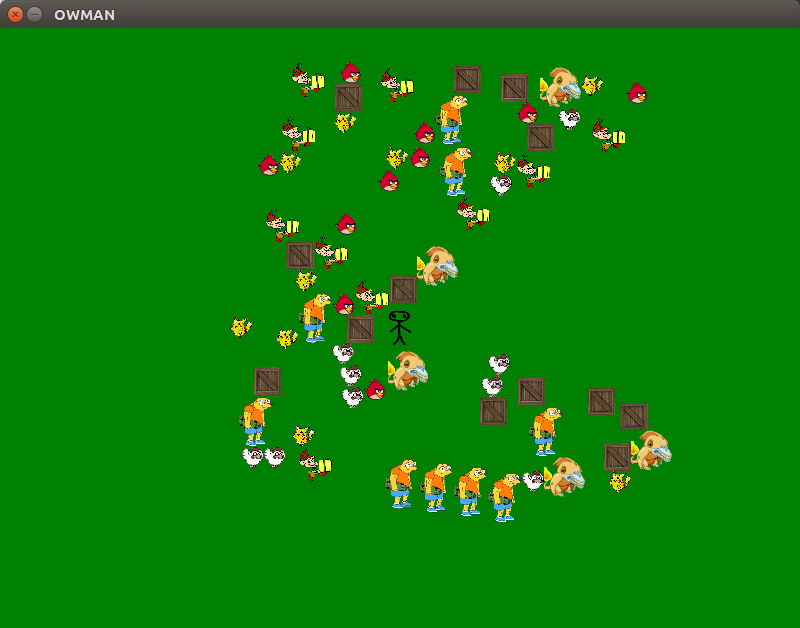
\includegraphics[scale=0.40]{size2.png}
	\caption{Window size = 2.}
	\label{fig:windowsize2}
\end{figure}

\begin{figure}[H]
	\centering
	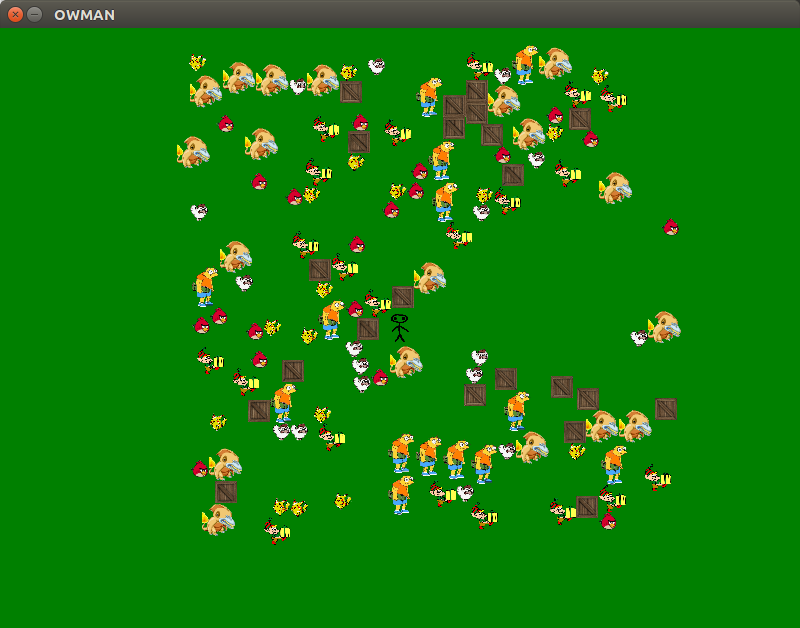
\includegraphics[scale=0.40]{size3.png}
	\caption{Window size = 3.}
	\label{fig:windowsize3}
\end{figure}

We have found that a window size of three is a good balance between performance and playability. Maybe four for high resolution screens

\begin{table}[H]
	\centering
	
    \begin{tabular}{|l|l|l|}
        \hline
        Window size & CPU & RAM    \\ \hline
        1           & ~1\% &  70.3MB \\ 
        2           & ~2\% &  70.3MB \\
        3			& ~4\% &  70.4MB \\
        4			& ~6\% &  70.6MB \\
        5			& ~9\% &  72.7MB \\
        6			& ~12\% & 74.4MB \\
        10			& ~24\% & 85.0MB \\
        \hline
    \end{tabular}
    \caption{Performance tests.}
\end{table}

The CPU consumption is highly dependent on the window size. We have measured that most of the CPU consumption is drawn at the drawing stage. The CPU consumption of the physics simulation is only a small part and the consumption of the other subsystems are negligible.

A big part (around half of the total) of the time spent during the drawing stage relies in matrix operations. I think there might be a slight margin of improvement in these matrix operations but not much.

Speaking about RAM consumption, the amount of RAM used increases very slowly compared to CPU. That is indeed the prove that our resource manager is taking care of duplicates.

\begin{figure}[H]
	\centering
	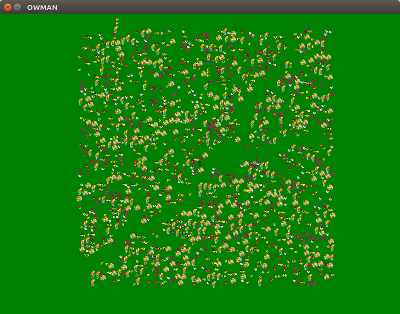
\includegraphics[scale=0.78]{size10.png}
	\caption{Window size = 10.}
	\label{fig:windowsize10}
\end{figure}



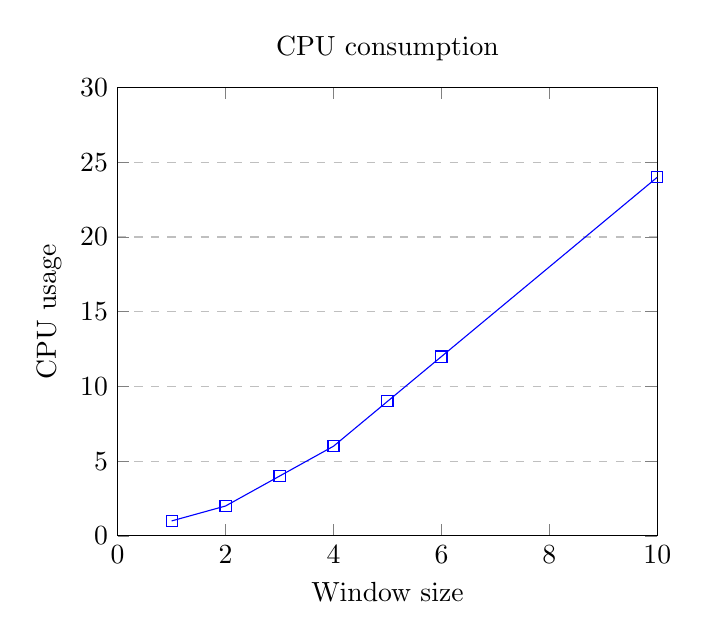
\begin{tikzpicture}
\begin{axis}[
    title={CPU consumption},
    xlabel={Window size},
    ylabel={CPU usage},
    xmin=0, xmax=10,
    ymin=0, ymax=30,
    xtick={0, 2, 4, 6, 8, 10},
    ytick={0, 5, 10, 15, 20, 25, 30},
    legend pos=north west,
    ymajorgrids=true,
    grid style=dashed,
]
 
\addplot[
    color=blue,
    mark=square,
    ]
    coordinates {
    (1, 1)(2, 2)(3, 4)(4, 6)(5, 9)(6, 12)(10, 24)
    };
 
\end{axis}
\end{tikzpicture}

By observing the graph, we can notice that the asymptotic cost is close to linear but not exactly. It might be something between linear and quadratic. That is a great achievement considering that the number of entities grows like O($(2n+1)^2$), that is highly quadratical (\emph{n} is the window size).

\section{Conclusion}

We have developed a game engine that supports big worlds. The performance is good, so it could be ported to mobile platforms (we have carefully chosen the dependencies for this purpose). We wanted to create a engine that would show how to overcome the technological challenges of big world games and I think that the goal has been accomplished.

In addition of creating the engine, we have been able to create a demo that tests the engine intensively. Thanks to this, we have proved that our engine is stable and, apparently, has no bugs.

We have successfully integrated graphics and physics.

Physics simulation is accurate thanks to the, moving the origin of coordinates, strategy. We have wrapped a particular physics engine but all the concepts used are applicable to any other physics engine.

We have implemented a small render engine. The reader of this article would learn how to implement a graphics system that has to cooperate with the resource manager to overcome the limitations of multithreading with OpenGL. Also, I have learned the basics of modern OpenGL programming and I have applied them.

Also, we have implemented a resource manager that could be used in other types of applications, not only videogames. Our resource manager is easy to extend. Avoiding race conditions has been a difficulty and we have successfully dealt with it.

The world streamer implementation works fine and our architecture would allow to create new implementations and swap between them easily. The world streamer is configurable, so it can be adapted to the hardware capabilities.

It was not a main requirement but we also managed so the modifications of the world are persistent. 

The code is well documented using doxygen syntax. Hopefully, any developer who is interested in learning or contributing could understand the code and extend the engine.

In my opinion world streaming is an interesting topic in the field of videogames. I think open world videogames will keep being among the most popular videogames. Up to now, successful open world videogames have come from very important companies that can make great investments. From my point of view, open world games are a difficult target for small companies and indie developers. Not only because the implementation of an appropriate engine is a lot of work, but also because a lot of content and resources have to be produced. But if the proper tools become available to them, that target will get feasible. Also, procedural generation could help developers to fill the world with great content. I think in some years the number of available tools for making open world games will grow and they will be accessible for anybody. I hope to see some indie open world games in a few years.

\section{Update: animation system}
\label{"sec:animationsystem"}

The new animation system I have implemented extends the engine and adds some complexity. Also, implementing this feature forced me to refactor the code. Now the engine is performing better (in terms of loading times), more stable and better organized.

The animation system is implemented from scratch. The animations are based in frames.

We have created a custom file format based in XML for representing sprites. Sprites can have multiple animations. The structure of these sprite files is represented in the following UML diagram.

\begin{figure}[H]
	\centering
	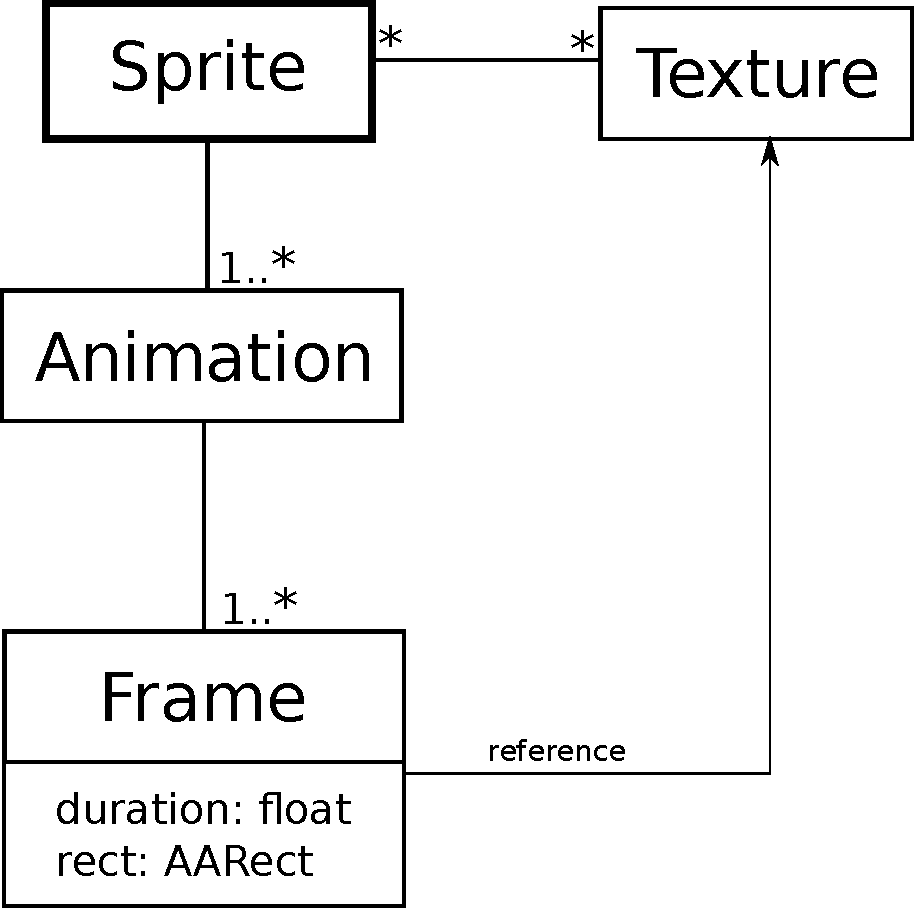
\includegraphics[scale=0.4]{sprite_uml.pdf}
	\caption{UML diagram}
	\label{fig:spriteuml}
\end{figure}

As you can see, one sprite has at least one animation and each animation has at least one frame. Frames have associated a duration and a rectangular region in a texture. Having the possibility to refer to a specific region of a texture allows us to use sprite sheets.

There are a lot of sample sprites in the \emph{bin/sprites} directory. This is a fragment of the sprite that we use as our main character:

\begin{minted}{xml}
<sprite>
	
	<textures>
		<tex id="sp1">pokemon_red_pj.png</tex>
	</textures>
	
	<animations>
	
		<anim id="stand_down">
			<frame>
				<tex>sp1</tex>
				<rect>
					<x>32</x> <y>0</y>
					<w>32</w> <h>32</h>
				</rect>
				<time>1</time>
			</frame>
		</anim>
		
		...
		
		<anim id="walking_up">
			<frame>
				<tex>sp1</tex>
				<rect>
					<x>0</x> <y>96</y>
					<w>32</w> <h>32</h>
				</rect>
				<time>0.2</time>
			</frame>
			<frame>
				<tex>sp1</tex>
				<rect>
					<x>32</x> <y>96</y>
					<w>32</w> <h>32</h>
				</rect>
				<time>0.15</time>
			</frame>
			<frame>
				<tex>sp1</tex>
				<rect>
					<x>64</x> <y>96</y>
					<w>32</w> <h>32</h>
				</rect>
				<time>0.2</time>
			</frame>
		</anim>
		
	</animations>

</sprite>


\end{minted}

It is useful to have an id for every animation, so it's straight forward to set an animation programmatically. If we wish to make an sprite which is not animated, we can make an animation with only one frame, since animations loop by default.

In the following diagram we try to represent the mechanism we use in order to load and display sprites.

\begin{figure}[H]
	\centering
	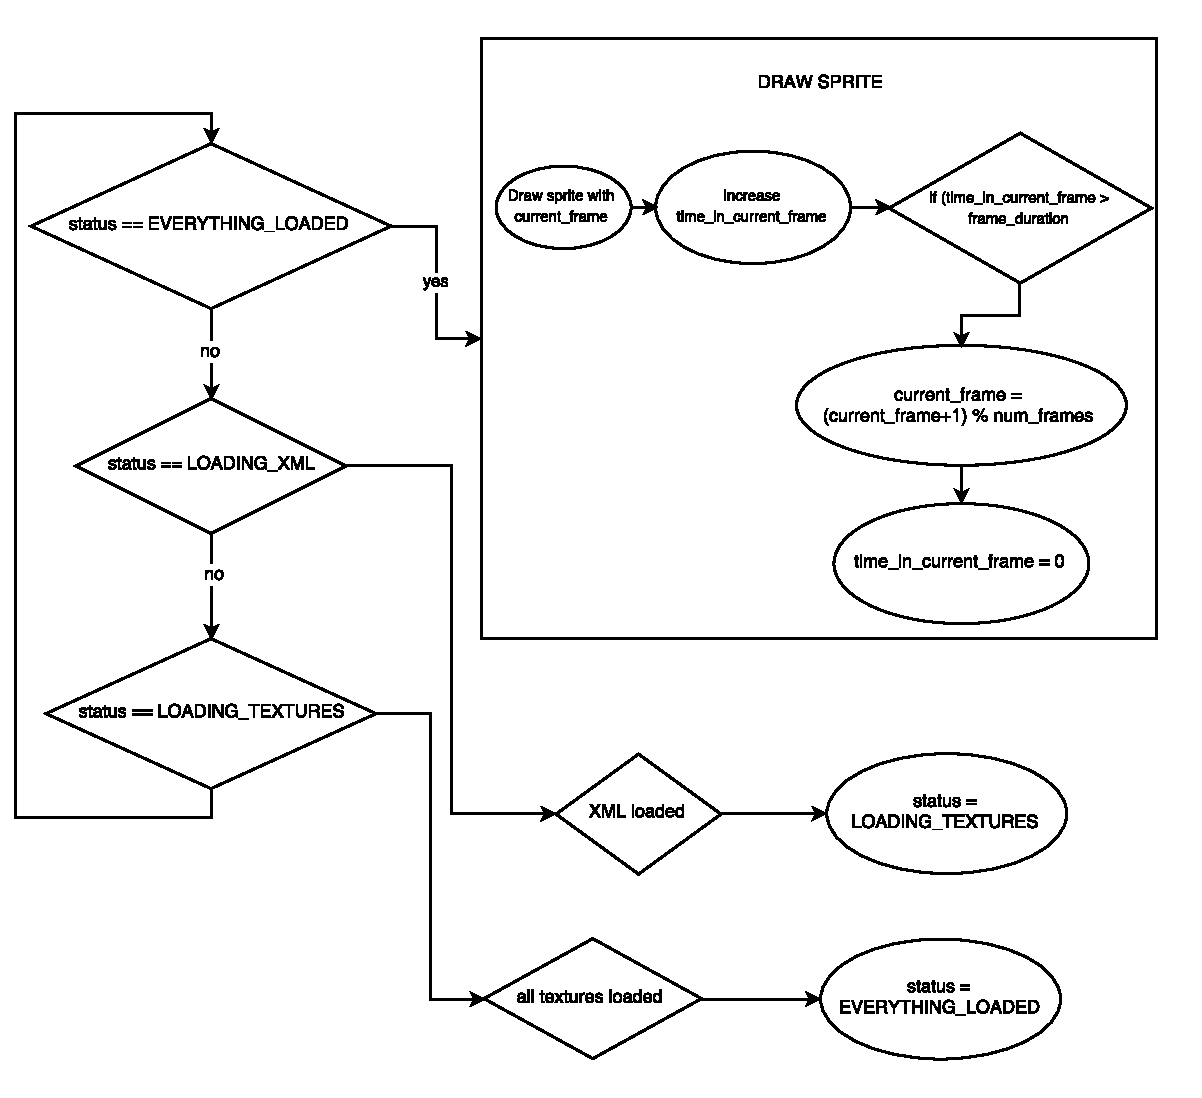
\includegraphics[scale=0.8]{sprite_loading.pdf}
	\caption{Flow chart of the sprite's loading process}
	\label{fig:spriteloading}
\end{figure}

Now there are more steps than when we had just static images. We need to read the XML of each sprite and from that file obtain the textures that must be loaded.

In the same way we made sure that no texture is twice in memory, we want to make sure no sprite is twice in memory. The class \emph{Sprite} contains the data which is common to all the entities using it. And the class \emph{SpriteStatus} only keeps track of the current status of the animation. That is, the current frame and the time spent in the current frame.

\begin{figure}[H]
	\centering
	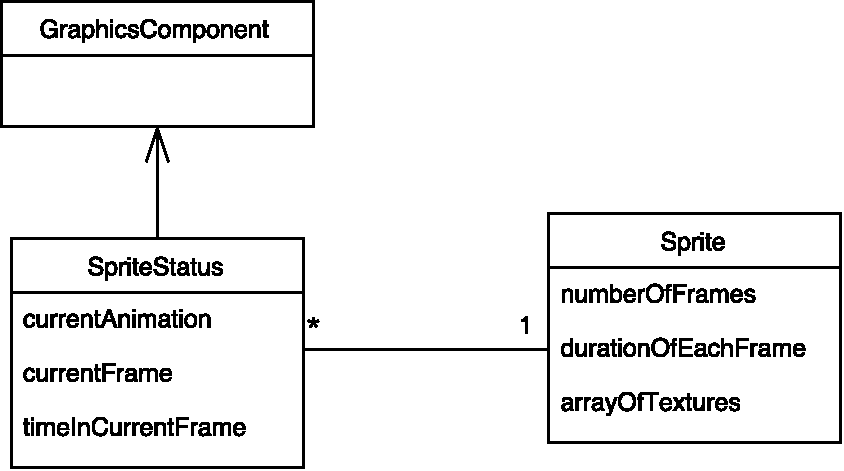
\includegraphics[scale=0.7]{sprite_status_uml.pdf}
	\caption{UML representation of the \emph{Sprite} and \emph{SpriteStatus} classes}
	\label{fig:spritestatusuml}
\end{figure}

In order to test the animation system I have created a new automatic world generation script. You can find it in "\emph{bin/world\_gens}". This new generator makes better looking worlds. The world is made up of a big set of template cells (can be found at \emph{bin/cell\_templates}). Our generator takes as input a certain number of rows and columns and fills the world with randomly chosen cell templates. This is an example of what we have seen in \ref{sec:contentgen}. In this case we are making a mixture of manually generated content and automatically generated content.

\begin{figure}[H]
	\centering
	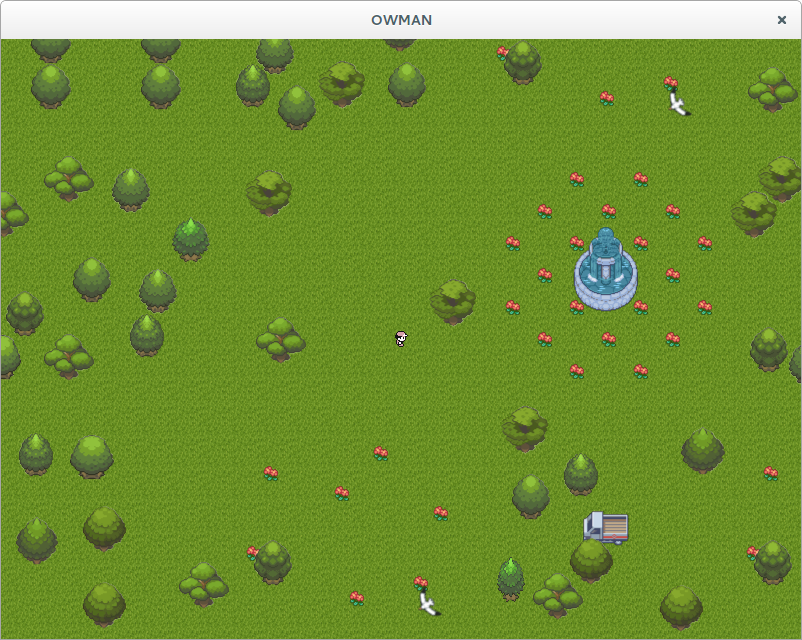
\includegraphics[scale=0.5]{anim_screenshot.png}
	\caption{Screenshot of one generated world}
	\label{fig:animscreenshot}
\end{figure}

In terms of performance we have performed the same tests we did and it seems that the animation system has not affected at all. The bottleneck keeps being the rendering stage.

\section{Future extensions}

I have taken the development of this game engine as a hobby. I pretend to continue the development in my spare time.

These are some of the features that I would like to get implemented.

\begin{itemize}
	
	\item \textbf{Scripting:} I have already started working on this feature. Right now, implementing game logic is really difficult. Since the beginning, the game logic was intended to be done by scripting. When this feature got implemented, I would consider the game engine usable to make some real games. I want to embed the Lua programming language.
	
	\item \textbf{World editor tool:} Right now, everything has to be done by editing text files. It would be great to have a tool that allows to edit the world and manage the assets. That would make the engine friendlier to use.
	
	\item \textbf{Sound:} No game is complete without sound.
	
	\item \textbf{World description data compression:} If you generate a very big world the \emph{world\_folder} gets flooded of small cell files. Getting these files packed in a single compressed file would save a lot of space and would make the \emph{world\_folder} easier to manage.
	
\end{itemize}

\section{License}

The developed software is open source. It is licensed under the MIT License.

The project is hosted in a public repository:\newline \url{https://github.com/tuket/OWMAN}.

\section{Tools and dependencies}

\subsection{Used tools}

\begin{itemize}

\item{\textbf{Code::Blocks.}} Used as the main IDE (integrated development environment).
\newline
\url{www.codeblocks.org}

\item{\textbf{Doxygen.}} Automatic generation of documentation from code coments.
\newline
\url{www.doxygen.org}

\item{\textbf{Apitrace.}} OpenGL debugger.
\newline
\url{apitrace.github.io}

\end{itemize}

\subsection{Dependencies}

\begin{itemize}

\item{\textbf{Boost FileSystem.}} Allows accessing the file system.
\newline
\url{www.boost.org/libs/filesystem}

\item{\textbf{OpenGL.}} Graphics API.
\newline
\url{www.opengl.org}

\item{\textbf{SDL2.}} As window manager.
\newline
\url{www.libsdl.org}

\item{\textbf{RapidXML.}} For parsing XML and modifiying the tree.
\newline
\url{rapidxml.sourceforge.net}

\item{\textbf{Box2d.}} As the physics engine.
\newline
\url{box2d.org}

\item{\textbf{POSIX Threads.}} For creating threads.
\newline
\url{pubs.opengroup.org/onlinepubs/7908799/xsh/pthread.h.html}

\item{\textbf{SOIL.}} A small library that allows to load textures.
\newline
\url{www.lonesock.net/soil.html}

\item{\textbf{GLEW.}} A library that defines the OpenGL extensions.
\newline
\url{glew.sourceforge.net}

\item{\textbf{GLM.}} A mathematics library for OpenGL.
\newline
\url{http://glm.g-truc.net}
\end{itemize}


\bibliography{tfg}

\begin{thebibliography}{99}

\bibitem{bestselling}
	\hypertarget{bestselling}
	List of the best-selling videogames.
	\newline
	\url{http://en.wikipedia.org/wiki/List_of_best-selling_video_games#All_platforms}
	
\bibitem{worldbilas}
	\hypertarget{worldbilas}
	The Continuous World of Dungeon Siege - Scott Bilas.
	\newline
	\url{http://scottbilas.com/files/2003/gdc_san_jose/continuous_world_paper.pdf}
	
\bibitem{rockstar}
	\hypertarget{rockstar}
	Technical leads Adam Fowler and Phil Hooker take us through the technology powering GTA V.
	\newline
	\url{http://www.develop-online.net/studio-profile/inside-rockstar-north-part-3-the-tech/0184140}
	
\bibitem{gta1}
	\hypertarget{gta1}
	GTA article at Wikipedia.
	\newline
	\url{http://en.wikipedia.org/wiki/Grand_Theft_Auto_%28video_game%29}

\bibitem{earnings}
	\hypertarget{earnings}
	Top 10 highest grossing videogames of all time.
	\newline
	\url{http://www.businessinsider.com/here-are-the-top-10-highest-grossing-video-games-of-all-time-2012-6?op=1}
	
\bibitem{multiopengl}
	\hypertarget{multiopengl}
	Stack Overflow post discouraging multithreaded rendering with OpenGL.
	\newline
	\url{http://stackoverflow.com/questions/11097170/multithreaded-rendering-on-opengl}
	
\bibitem{shader}
	\hypertarget{shader}
	Shaders on Wikipedia.
	\newline
	\url{http://en.wikipedia.org/wiki/Shader}
	
\bibitem{glsl}
	\hypertarget{glsl}
	GLSL on Wikipedia.
	\newline
	\url{http://en.wikipedia.org/wiki/OpenGL_Shading_Language}
	
\bibitem{shadtut}
	\hypertarget{shadtut}
	GLSL tutorial
	\newline
	\url{http://www.lighthouse3d.com/tutorials/glsl-tutorial}
	
\bibitem{glmodtut}
	\hypertarget{glmodtut}
	Modern OpenGL tutorial.
	\newline
	\url{https://open.gl}
	
\bibitem{learngl}
	\hypertarget{learngl}
	Learn OpenGL.
	\newline
	\url{http://www.learnopengl.com}
	
\bibitem{glm}
	\hypertarget{glm}
	GLM official webpage.
	\newline
	\url{http://glm.g-truc.net}

\bibitem{sdl}
	\hypertarget{sdl}
	SDL official webpage.
	\newline
	\url{https://www.libsdl.org}
	
\bibitem{soil}
	\hypertarget{soil}
	SOIL official webpage.
	\newline
	\url{http://www.lonesock.net/soil.html}
	
\bibitem{box2d}
	\hypertarget{box2d}
	Box2D official webpage.
	\newline
	\url{http://box2d.org}
	
\bibitem{workqueue}
	\hypertarget{workqueue}
	Multithreaded Work Queue in C++.
	\newline
	\url{http://vichargrave.com/multithreaded-work-queue-in-c}
	
\bibitem{rapidxmlbug}
	\hypertarget{rapidxmlbug}
	Solution to RapidXml bug at StackOverflow.
	\newline
	\url{http://stackoverflow.com/questions/14113923/rapidxml-print-header-has-undefined-methods}

\bibitem{gamecodingcomplte}
	\hypertarget{gamecodingcomplte}
	Game Coding Complete - Mike McShaffry and David Graham.
	\newline
	\url{http://www.mcshaffry.com/GameCode}

\bibitem{gameenginearchitecture}
	\hypertarget{gameenginearchitecture}
	Game Engine Architecture - Jason Gregory
	\newline
	\url{http://www.gameenginebook.com}

\bibitem{ttmathlink}
	\hypertarget{ttmathlink}
	TTMath library
	\newline
	\url{http://www.ttmath.org/}
	
\bibitem{levelgame}
\hypertarget{levelgame}
Level (video gaming) - Wikipedia
\newline
\url{https://en.wikipedia.org/wiki/Level_%28video_gaming%29}
	
\bibitem{retrocitysmall}
\hypertarget{retrocitysmall}
Steam discussion about the small size of Retro City Rampage
\newline
\url{http://steamcommunity.com/app/204630/discussions/0/882962698536189638/}
	
\end{thebibliography}


\end{document}

